\section{Kinematics}

In kinematics, we are interested in describing the motion of particles. In this section we will discuss the motion of particles in one or two dimensions. 

\subsection{Position}

The position of a particle can be modelled as a function of time. Because the motion of the particle may involve more than on dimension, a vector representation is adopted. 

\begin{definition}{(\textbf{Position})}
\textit{The position of a particle $p$ at time $t$ is denoted as $\vec{r}(t)$. For example, assuming that the motion takes place in two dimension, $\vec{r}(t)$ is}
\begin{equation*}
    \vec{r}(t) = x(t) \hat{i} + y(t) \hat{j} = \langle x(t), y(t) \rangle.
\end{equation*}
\textit{More generally, for $n$ dimensional motion, we write}
\begin{equation}
    \vec{r}(t) = \langle r_1 (t), r_2 (t), \ldots r_n (t) \rangle.
\end{equation}
\end{definition}

Since the initial position of the particle is often known (the origin), we denote the initial position of the particle as $\vec{r}_0$. We can then immediately analyze the distance travelled and the net displacement, by analyzing the displacement and velocity of the particle.

\subsection{Displacement and Velocity}

\begin{definition}{(\textbf{Displacement})}
\textit{The displacement $\vec{s}(t)$, sometimes written as $\Delta \vec{r}(t)$, of a particle $p$ at time $t$ is the difference between the current position of particle $p$ at time $t$ $\vec{r}(t)$ and the origin $\vec{r}_0$. }
\begin{equation}
    \vec{s}(t) = \Delta \vec{r}(t) = \vec{r}(t) - \vec{r}_0
\end{equation}
\textit{measured in \textbf{metres} ($m$).}
\end{definition}

We shall discuss the speed and distance once we have defined velocity. This is because we note that the displacement experienced by a particle is zero if the particle returns to its initial point, while the distance covered by the particle along this path is not zero. Now we need to introduce the concepts of \textit{instantaneous} velocity and \textit{averaged} velocity.

\begin{definition}{(\textbf{Velocity})}
\textit{The instantaneous velocity $\vec{v}(t)$ of a particle $p$ is defined as the rate of change of displacement. Hence, instantaneous velocity can only be defined mathematical (we know it exists physically but cannot measure it experimentally).}
\begin{equation}
    \vec{v}(t) = \lim_{\Delta t \rightarrow 0} \frac{\vec{s}(t + \Delta t)}{\Delta t} = \frac{\mathop{\mathrm{d}\vec{s}(t)}}{\mathop{\mathrm{d}t}}
\end{equation}
\textit{measured in \textbf{metres per second} ($ms^{-1}$).}
\end{definition}

The averaged velocity $\overline{\vec{v}}$ is simply calculated by determining the change in displacement over a time interval $\Delta t = t_1 - t_0$ and calculating the ratio:
\begin{equation}
    \overline{\vec{v}} = \frac{\vec{s}(t_1) - \vec{s}(t_0)}{\Delta t}
\end{equation}

\subsection{Displacement-Time Graphs}

It is often useful to represent the motion of a particle using a graph, for example plotting displacement against time, also known as \textit{displacement-time} (\textit{s-t}) graphs. We can then use the graph to find the instantaneous velocity of the particle or the distance travelled. The gradient of a displacement-time graph is the velocity of the particle and the distance travelled can be found by adding the change in displacements of where the velocity is zero or displacement is zero. To graphically find the instantaneous velocity of the particle at time $t$, we draw a tangent to the curve at time $t$. The velocity at $t$ is then the gradient of the tangent. 


\begin{figure}[h!]
    \centering
    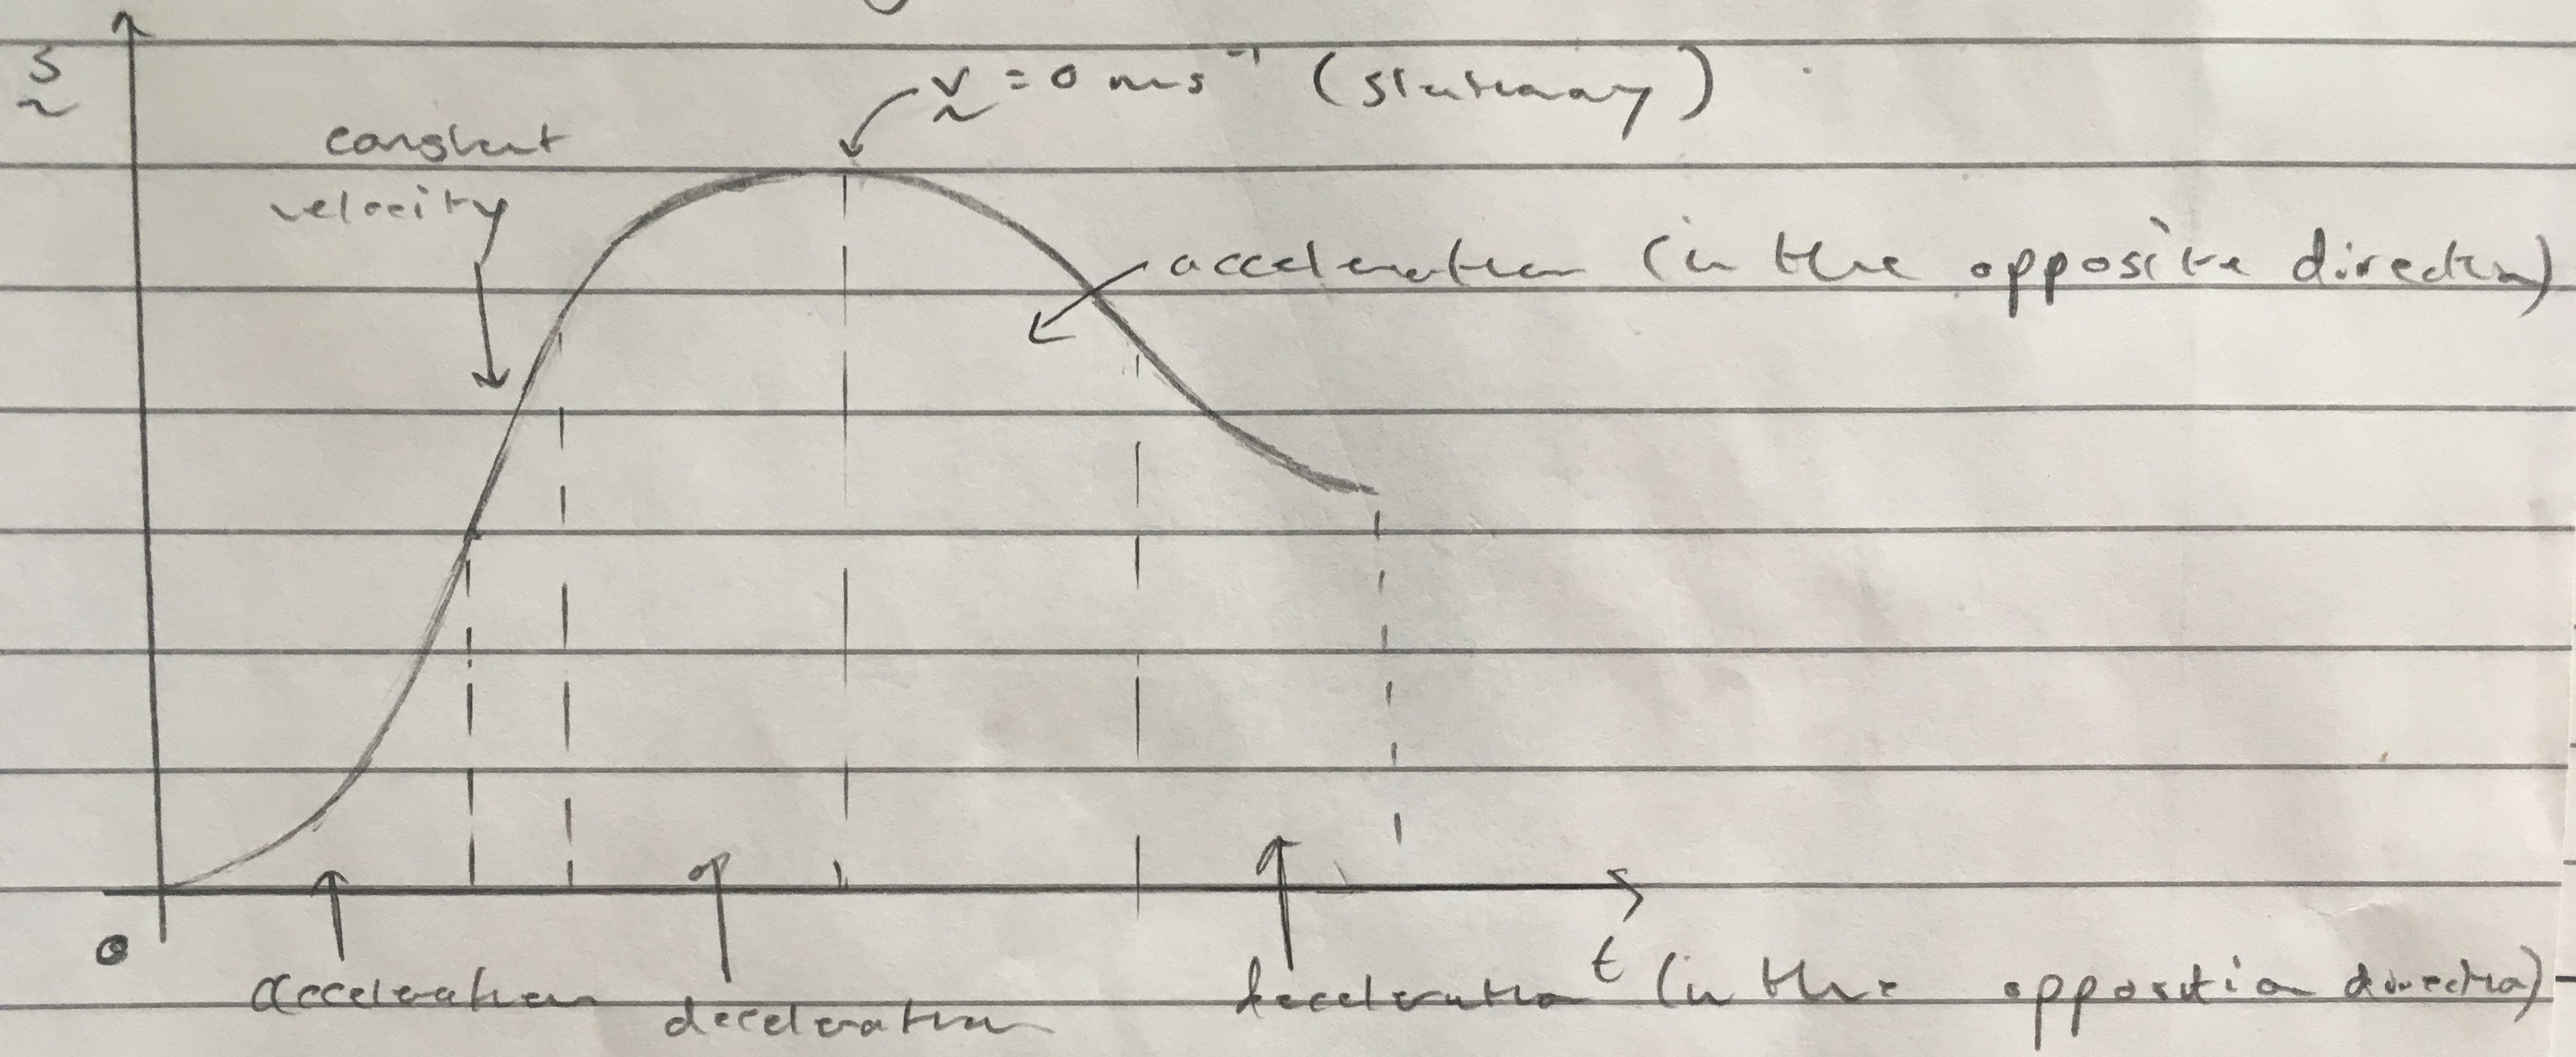
\includegraphics[scale=0.1]{notes/images/Displacement-Time-Graph.JPG}
    \caption{A \textit{s-t} graph}
\end{figure}
\FloatBarrier

\subsection{Distance and Speed}

The concept of velocity is associated with displacement, the concept of speed is associated with the distance travelled by the particle. Hence velocity is a vector quantity and speed is a scalar quantity. We note that due to the \textit{fundamental theorem of calculus} that 
\begin{equation*}
    \vec{s}(t) = \int \vec{v}(t) \mathop{\mathrm{d}t} 
\end{equation*}

\begin{definition}{(\textbf{Distance})}
\textit{The distance travelled $x(t)$, measured in metres ($m$),by the particle $p$ at time $t$ is given by }
\begin{equation}
    x(t) = \sum_{i = 1} ^ n \left|\int_{t_{i-1}}^{t_{i}} \vec{v}(t) \mathop{\mathrm{d}t}\right|
\end{equation}
\textit{where for all $i = 1, 2, \ldots, n$ we have $\vec{v}(t_i) = \vec{0}$ or $\vec{s}(t_i) = \vec{0}$ and $0 \leq t_1 < t_2 < \ldots < t_n \leq t$.}
\end{definition}
\noindent From our definition of distance, we can now define average speed. 
\begin{definition}{(\textbf{Average Speed})}
\textit{The average speed $\overline{v}(t)$, measured in metres per second ($ms^{-1}$), of a particle $p$ at time $t$ is given by}
\begin{equation}
    \overline{v}(t) = \frac{x(t)}{t}
\end{equation}
\end{definition}

\subsection{Distance-Time Graphs}

For a similar motivation to \textit{s-t} graphs, we often plot a distance against time graph, also known as \textit{displacement-time} (\textit{x-t}) graphs. We can use the graph to find the instantaneous speed, using a similar method for finding the instantaneous velocity and finding the distance travelled. To find the distance travelled we use the method of dissection to analyze sections of the journey. We then find the distance travelled in each section and sum up the distances from each section in the provided time ranges, to find the total distance travelled. 

\begin{figure}[h!]
    \centering
    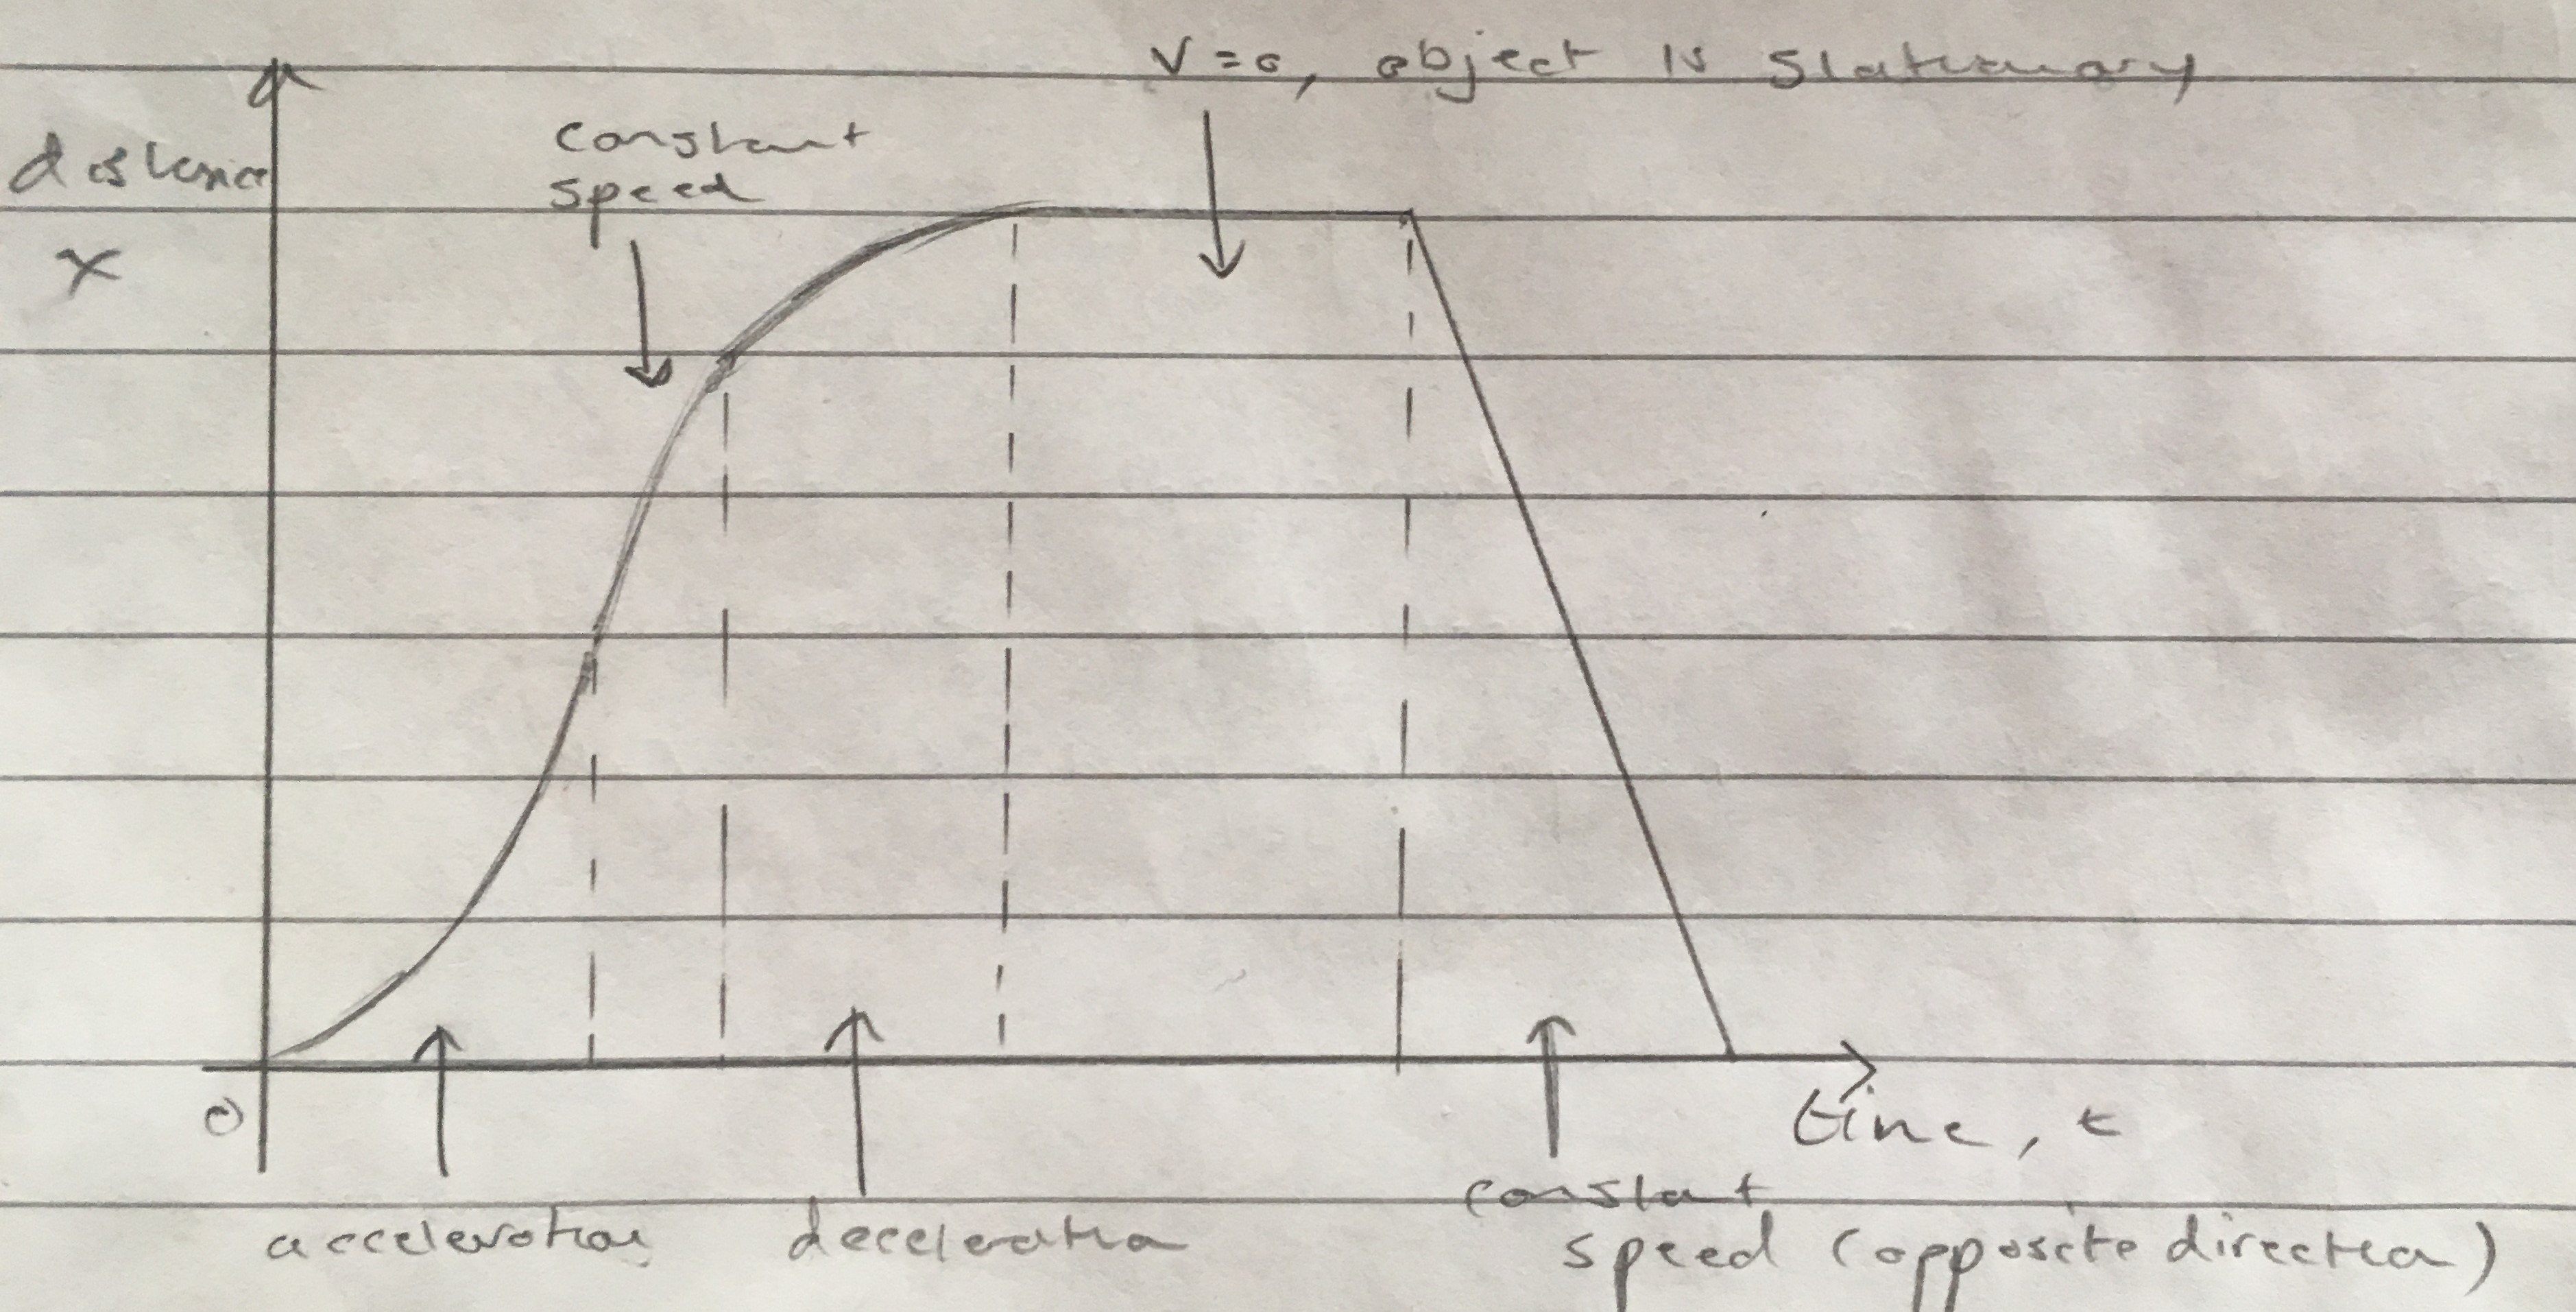
\includegraphics[scale=0.1]{notes/images/Distance-Time-Graph.jpg}
    \caption{A \textit{x-t} graph}
\end{figure}
\FloatBarrier

\subsection{Acceleration}

The last kinematic attribute of particle motion involves the determination of whether the instantaneous velocity $\vec{v}(t)$ of the particle changes as a function of time.

\begin{definition}{(\textbf{Acceleration})}
\label{def:acceleration}
\textit{The instantaneous acceleration $\vec{a}(t)$ of a particle $p$ is defined as the rate of change of the instantaneous velocity $\vec{v}(t)$: }
\begin{equation}
 \vec{a}(t) = \frac{\mathop{\mathrm{d}\vec{v}(t)}}{\mathop{\mathrm{d}t}}  
\end{equation}
\textit{measured in \textbf{metres per second squared} ($ms^{-2}$)}
\end{definition}
Note that the instantaneous acceleration of a particle can also be defined in terms of the section time derivative of its instantaneous displacement $\vec{s}(t)$.
\begin{equation*}
    \vec{a}(t) = \frac{\mathop{\mathrm{d}^2\vec{s}(t)}}{\mathop{\mathrm{d}t^2}}
\end{equation*}
Negative acceleration, or acceleration in the opposite direction to motion is usually called deceleration, however this might depend on the context of the scenario. 

\subsection{Velocity-Time Graphs}

For a similar motivation to \textit{s-t} and \textit{x-t} graphs, we often plot a velocity against time graph, also known as \textit{velocity-time} (\textit{v-t}) graphs. We can use the graph to find the instantaneous acceleration, using a similar method for finding the instantaneous velocity, and finding the displacement. To find the displacement using a \textit{v-t} graphs, we use the fundamental theorem of calculus, recalling that
\begin{equation*}
    \vec{s}(t) = \int \vec{v}(t) \mathop{\mathrm{d}t}.
\end{equation*}
Hence the area under a \textit{v-t} graph with bounds zero and $T$ seconds is equivalent to the displacement at time $T$. In A2 Physics we're not allowed to directly work with integrals, hence we must use the trapezium rule to estimate the area under the graph.  

\begin{figure}[h!]
    \centering
    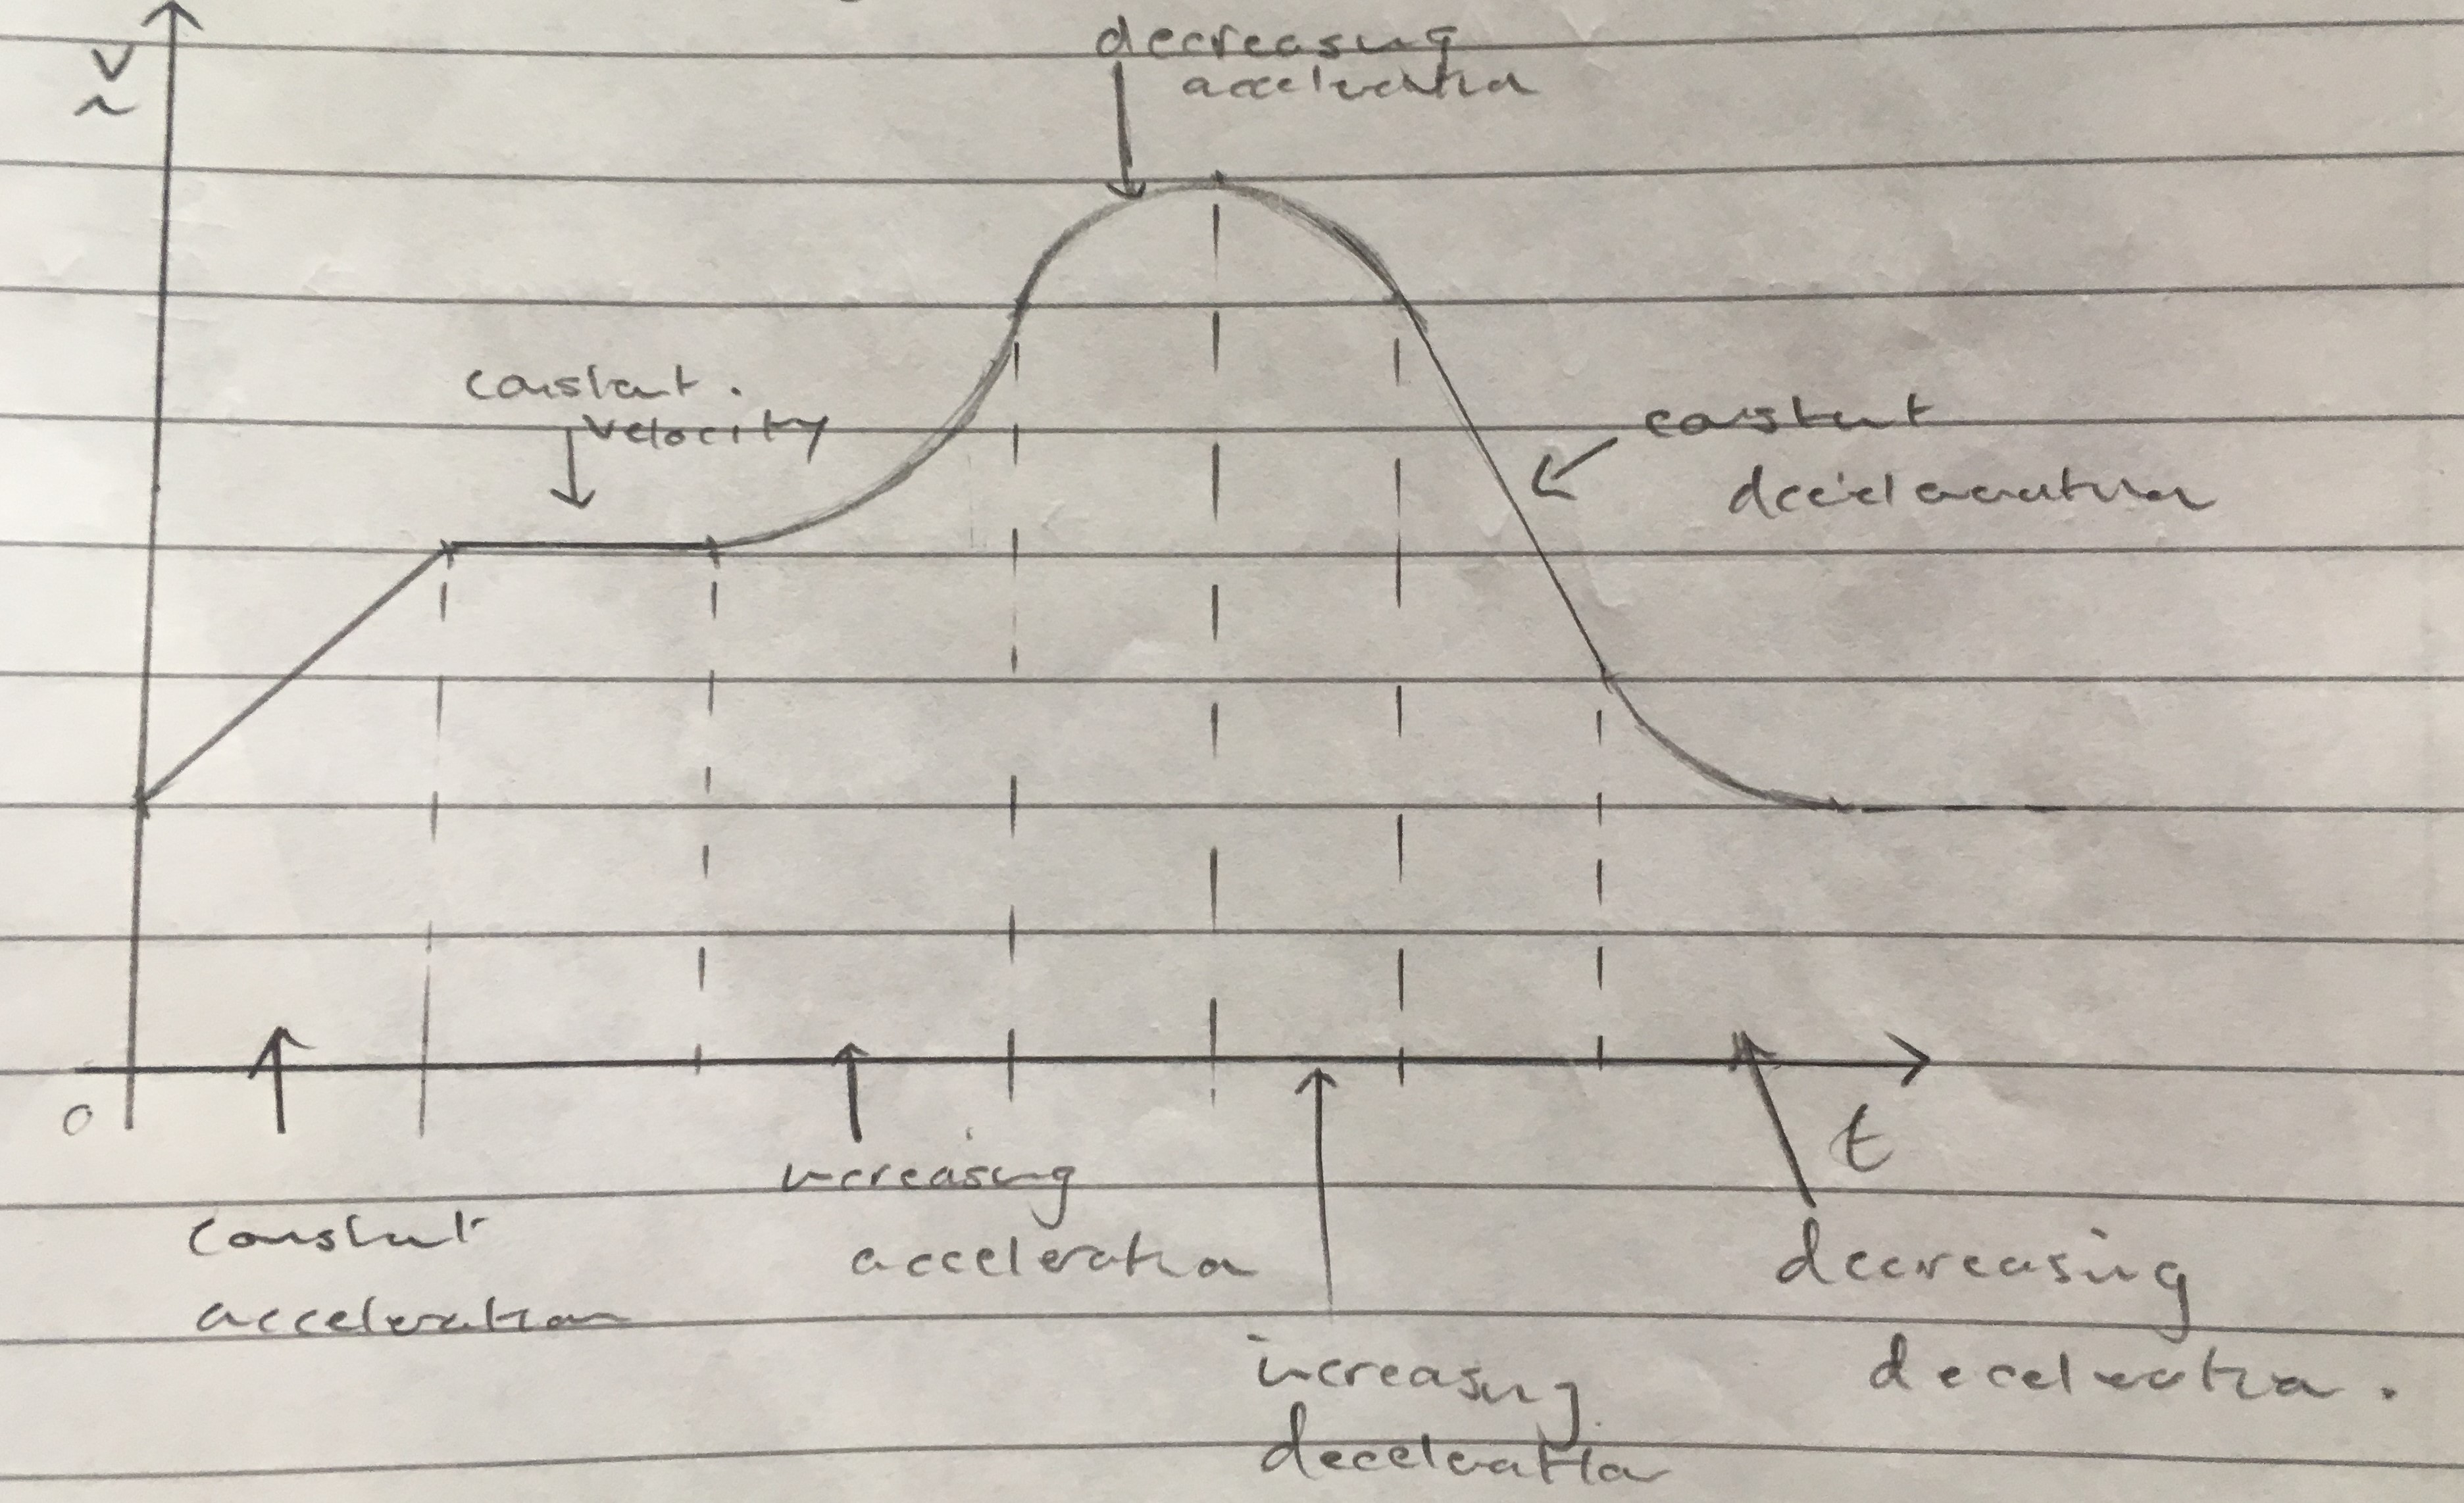
\includegraphics[scale=0.1]{notes/images/Velocity-Time-Graph.jpg}
    \caption{A \textit{v-t} graph}
\end{figure}
\FloatBarrier

\subsection{Equations of Motion}
\label{subsection:equations-of-motion}

This section will discuss one dimensional equations of motion for constant acceleration. It would be correct to say that no object has ever traveled in one-dimension with a constant acceleration anywhere in the universe at any time (due to relativity). However, it is useful to approximate real situations with models based on ideal situations (i.e constant acceleration). We will derive new equations that can be used to describe the motion of an object in terms of its three kinematic variables: acceleration $\vec{a}$, velocity $\vec{v}$, initial velocity $\vec{u}$, displacement $\vec{s}$ and time $t$. Since we are dealing with vector quantities, the use of vector calculus is necessary. 

By considering the definition of acceleration (see definition \ref{def:acceleration}), the fundamental theorem of calculus and assuming acceleration is constant, we get the velocity-time equation for constant acceleration, the so-called \textit{first equation of motion} (see equation \ref{eq:first-equation-of-motion}):
\begin{align*}
    \vec{a} &= \frac{\mathop{\mathrm{d}\vec{v}}}{\mathop{\mathrm{d}t}} \\
    \mathop{\mathrm{d}\vec{v}} &= \vec{a}\mathop{\mathrm{d}t} \\
    \int_{\vec{u}}^{\vec{v}} \mathop{\mathrm{d}\vec{v}} &= \int_0^t \vec{a}\mathop{\mathrm{d}t} \\
    \vec{v} - \vec{u} &= \vec{a}t,
\end{align*}
giving, 
\begin{equation}
    \label{eq:first-equation-of-motion}
    \vec{v} = \vec{u} + \vec{a}t.
\end{equation}

Again by definition, velocity is the first time derivative of displacement. Applying the fundamental theorem of calculus to this gives the displacement-time equation for constant acceleration, also known as the \textit{second equation of motion} (see equation \ref{eq:second-equation-of-motion})
\begin{align*}
    \vec{v} &= \frac{\mathop{\mathrm{d}\vec{s}}}{\mathop{\mathrm{d}t}} \\
    \mathop{\mathrm{d}\vec{s}} &= \vec{v}\mathop{\mathrm{d}t} \\
    \int_0^{\vec{s}} \mathop{\mathrm{d}\vec{s}} &= \int_0^t (\vec{u} + \vec{a}t) \mathop{\mathrm{d}t},
\end{align*}
evaluating the integral gives the second equation of motion,
\begin{equation}
    \label{eq:second-equation-of-motion}
    \vec{s}= \vec{u}t + \frac{1}{2}\vec{a}t^2.
\end{equation}

Unlike the first and second equations of motion, the \textit{third equation of motion} (see equation \ref{eq:third-equation-of-motion}), which relates velocity to displacement, cannot be obtained by reverse engineering the definitions of velocity or displacement. To do so, we need to consider the derivative of velocity with respect to displacement. 

\begin{equation*}
    \frac{\mathop{\mathrm{d}\vec{v}}}{\mathop{\mathrm{d}\vec{s}}} = \hspace{1mm} ?
\end{equation*}

To evaluate this derivative, we need to consider the chain rule. We note that the derivative above is equal to the product of acceleration and the inverse of velocity, that is
\begin{align*}
    \frac{\mathop{\mathrm{d}\vec{v}}}{\mathop{\mathrm{d}\vec{s}}} &= \frac{\mathop{\mathrm{d}\vec{v}}}{\mathop{\mathrm{d}t}} \cdot \frac{\mathop{\mathrm{d}t}}{\mathop{\mathrm{d}\vec{s}}} \\
    &= \vec{a} \cdot \frac{1}{\vec{v}}
\end{align*}

We should note that the reciprocal of a vector is mathematically speaking impossible, instead (in linear algebra) we consider the associated \textit{reciprocal vector} of $\vec{a}$, denoted $\vec{a}^{-1}$ such that $\vec{a} \cdot \vec{a}^{-1} = \vec{1}$. The next step is the separation of variables and then to integrate them. 

\begin{align*}
    \frac{\mathop{\mathrm{d}\vec{v}}}{\mathop{\mathrm{d}\vec{s}}} &= \vec{a} \cdot \frac{1}{\vec{v}} \\
    \vec{v} \cdot \mathop{\mathrm{d}\vec{v}} &= \vec{a} \cdot \mathop{\mathrm{d}\vec{s}} \\
    \int_{\vec{u}}^{\vec{v}} \vec{v} \cdot \mathop{\mathrm{d}\vec{v}} &= \int_0^{\vec{s}} \vec{a} \cdot \mathop{\mathrm{d}\vec{s}} \\
    \frac{1}{2}(\vec{v}\cdot \vec{v} - \vec{u} \cdot \vec{u}) &= \vec{a} \cdot \vec{s}
\end{align*}
The definition of the euclidean length of a vector $\vec{a}$, denoted $\| \vec{a} \|$, using dot product is $\| \vec{a} \| = \sqrt{\vec{a} \cdot \vec{a}}$, so we have 
\begin{equation}
    \label{eq:third-equation-of-motion}
    \| \vec{v} \|^2 = \| \vec{u} \|^2 + 2 \vec{a} \cdot \vec{s}.
\end{equation}
Alternatively, we could consider a one-dimensional model for each dimension in our model. For example, assuming that the motion takes places in two dimensions, we have
\begin{align*}
    v_x^2 &= u_x^2 + 2 a_x s_x, \\
    v_y^2 &= u_y^2 + 2 a_y s_y.
\end{align*}

We can now combine the three equations of motion to produce our so-called \textit{SUVAT} equations (shown below) where ``SUVAT'' is an acronym for the variables $\vec{s}$, $\vec{u}$, $\vec{v}$, $\vec{a}$ and $t$.
\begin{align}
    \vec{v} &= \vec{u} + \vec{a}t, \\
    \vec{s} &= \frac{1}{2}(\vec{u} + \vec{v})t, \\
    \vec{s} &= \vec{u}t + \frac{1}{2}\vec{a}t^2, \\
    \vec{s} &= \vec{v}t - \frac{1}{2}\vec{a}t^2, \\
    \| \vec{v} \|^2 &= \| \vec{u} \|^2 + 2\vec{a}\cdot \vec{s}.
\end{align}


\subsection{Free fall}

In physics, ``free fall'' is any motion of a body where gravity is the only force acting upon it. However the term is often used more loosely than the strict sense defined above. Thus, falling through an atmosphere without a deployed parachute is often referred to as \textit{free fall}. 

Newton's law of gravitation states that every body with mass attracts every other body in the universe  (see section ??). On earth, objects accelerate vertically downwards towards the centre of the earth due to this law. When an object is accelerating under ``gravity'', it is said to be in free fall (see above). The magnitude of the acceleration due to gravity, denoted by the symbol $\| \vec{g} \|$, is approximately $9.8$ $ms^{-2}$ on earth.   

In A2 Physics, we are required to know methods for determining this value. We will consider two experiments, the electromagnet and trap door method and the light gates method. 

\subsubsection{Electromagnet and Trap door}

An electromagnet holds a steel ball. When the current to the electromagnet is switch off, a timer is triggered as the magnet demagnetizes. When the magnet demagnetizes the ball is dropped. When the ball hits the trap door, the electrical contact is broken and the time stops. Applying the second equation of motion (under constant acceleration) we have  
\begin{equation}
    \vec{s} = \frac{1}{2}\vec{g}t^2.
\end{equation}
We can measure the displacement between the electromagnet and the trap door, so the only unknown left is the acceleration due to gravity $\vec{g}$. Rearranging the equation above, we can solve for $\vec{g}$.
\begin{equation}
    \vec{g} = \frac{2}{t^2}\vec{s}
\end{equation}
So we can just compute the magnitude of $\vec{g}$ to find an approximation to $\| \vec{g} \|$. The apparatus for this experiment is shown below. 

\subsubsection{Light Gates}

In theory, this method should be more accurate than the one described above, since light gates reduce the time delay. Place one light gate above another (vertically) with a known displacement $\vec{s}$ between them. Both light gates are then connected to a timer or data logger. A ball is dropped from through the first light gate triggering the timer to start. When the ball finally passes through the second light gate the timer stops. We can apply the same equation of motion we used in the method above to then find an approximate value of $\| \vec{g} \|$.


\subsection{Projectiles}

A projectile is any object that is cast, fired, flung, heaved, hurled or thrown. (This is an informal definition). The path of a project is called its \textit{trajectory}. Some examples of projects might include bullets, balls, rockets (after engine cut off), etc.

\begin{definition}{(\textbf{Projectile})}
\textit{A projectile is any object that once projected continues in motion by its own inertia and is influenced by the downwards force of gravity.}
\end{definition}

That is not to say other forces do not exist, just that they are negligible or have minimal effect in comparison. Another essential characteristics of a projectile is that its future has already been determined. Some projectiles travel far enough to experience a variation in acceleration due to gravity, for example a rocket will experience a variation in $\| \vec{g} \|$ by approximately $\pm 0.05$ $ms^{-2}$. To distinguish between projectiles that experience this variation, we use the term \textit{simple projectile}. For the remaining problems, the term \textit{general projectile} is adopted. 

Every projectile problem is essentially two one-dimensional motion problems, considering motion in the $x$ and $y$ planes. The kinematic equations for a simple projectile are those of an object traveling with constant horizontal velocity and a constant vertical acceleration, hence the equations of motion discussed in section \ref{subsection:equations-of-motion} can be applied. 

The equations of motion for a simple projectile are as follows
\begin{align}
    \vec{a}_x &= 0 & \vec{a}_y &= \vec{g} \\
    \vec{v}_x &= \vec{u}_x & \vec{v}_y &= \vec{u}_y + \vec{g}t \\
    \vec{s}_x &= \vec{u}_x t & \vec{s}_y &= \vec{u}_y t + \frac{1}{2} \vec{g}t^2 \\
    \hspace{1mm} & \hspace{1mm} & \| \vec{v}_y \|^2 &= \| \vec{u}_y \|^2 + 2 \vec{g} \cdot \vec{s} 
\end{align}
Note that any vectors in the above equations only exists in $\mathbb{R}$ and $\vec{g} = - \| \vec{g} \|$. Having obtained the equations of motion for a simple projectile, we can consider the maximum range of a projectile based on it's initial angle with the horizontal (note that this case only works with a projectile that has an initial horizontal and vertical position of zero). Considering the horizontal position, we have
\begin{align*}
    \vec{r}_x &= \vec{r}_{0, x} + \vec{u}_x t + \frac{1}{2} \vec{a}_x t^2 \\
    &= 0 + (\| \vec{u} \| \cos \theta) t + 0 \\
    &= (\| \vec{u} \| \cos \theta) t,
\end{align*}
so the final horizontal position is given by, 
\begin{equation*}
    \vec{r}_{x, final} = (\| \vec{u} \| \cos \theta) t_{final}.
\end{equation*}
Considering the vertical position, we have
\begin{align*}
    \vec{r}_y &= \vec{r}_{0, y} + \vec{u}_y t + \frac{1}{2} \vec{a}_y t^2 \\
    &= (\| \vec{u} \| \sin \theta) t - \frac{1}{2} \| \vec{g} \| t^2,
\end{align*}
and if we consider when $\vec{r}_y = 0$ (the final vertical position), we have
\begin{align*}
    0 &= (\| \vec{u} \| \sin \theta) t - \frac{1}{2} \| \vec{g} \| t_{final}^2 \\
    t_{final} &= \frac{2(\| \vec{u} \| \sin \theta)}{\| \vec{g} \|}.
\end{align*}
Combining these two equations,
\begin{align}
    \vec{r}_{x, final} &= (\| \vec{u} \| \cos \theta) \frac{2(\| \vec{u} \| \sin \theta)}{\| \vec{g} \|} \\
    &= \frac{\| \vec{u} \|^2 \sin 2\theta}{\| \vec{g} \|}.
\end{align}
If we consider the maximum of $\sin 2\theta$, then we get $\theta = \frac{\pi}{4}$. Hence the maximum range of a projectile with $\vec{r}_0 = \vec{0}$, denoted $\vec{r}_{x, max}$, is 
\begin{equation}
    \vec{r}_{x, max} = \frac{\| \vec{u} \|^2}{\| \vec{g} \|}.
\end{equation}

\subsection{Frames of reference}

A frame of reference is defined by a set of \textbf{coordinate axes} $(x, y, z)$ at rest relative to a particular observer. The observer can express the \textbf{position}, \textbf{velocity} and \textbf{acceleration} of a particle \textbf{relative to this frame of reference}. We want to consider transformations of these quantities between different frames of reference. This is particularly important in the \textbf{theory of relativity} (in modern physics). 

So for example, let us consider one frame of reference $S$, fixed relative to the Earth and another frame of reference $S'$ fixed relative to a car moving with a constant velocity $\vec{v}$ relative to the Earth, as shown in figure ??. 


Suppose the origins $O$ and $O'$ coincide at time $t = 0$. A point $P$ has the position $\vec{r}$ at time $t$ in $S$ and $\vec{r}'$ in $S'$, so that
\begin{equation*}
    \vec{r}' = \vec{r} - \vec{v}t 
\end{equation*}
Now suppose that point $P$ is moving at a constant velocity $\vec{u}$ relative to the Earth, then by definition
\begin{equation*}
    \vec{u} = \frac{\mathop{\mathrm{d}\vec{r}}}{\mathop{\mathrm{d}t}},
\end{equation*}
so the velocity of the point $P$ relative to the car is 
\begin{equation*}
    \vec{u}' = \frac{\mathop{\mathrm{d}\vec{r}'}}{\mathop{\mathrm{d}t}} = \frac{\mathop{\mathrm{d}\vec{r}}}{\mathop{\mathrm{d}t}} - \vec{v} = \vec{u} - \vec{v}
\end{equation*}

%So generally, if we consider a frame of reference $S$, relative to the Earth with a velocity $\vec{u}$ and another frame of reference $S'$, relative to the Earth with a velocity $\vec{v}$ and assuming the origins $O$ and $O'$ coincide at time $t = 0$ and the point $P$ has the position $\vec{r}_0$ at time $t=0$, then it has the position $\vec{r}$ in $S$ at time $t$ and $\vec{r}'$ in $S'$, so that
%\begin{align*}
%    \vec{r} &= \vec{r}_0 - \int_0^t \vec{u} \mathop{\mathrm{d}t} \\
%    \vec{r}' &= \vec{r} - \int_0^t \vec{v} \mathop{\mathrm{d}t} \\
%    &= \vec{r}_0 - \int_0^t \vec{u} + \vec{v} \mathop{\mathrm{d}t}
%\end{align*}
    
Now as we mentioned earlier, transformations of quantities is one of the key considerations in reference frames. So lets consider the transformation of velocity and acceleration. So the velocity of the point $P$ is  (from the example above)
\begin{equation*}
    \vec{u}' = \vec{u} - \vec{v}.
\end{equation*}
Suppose the velocity of the car $\vec{v}$ is constant, but the point $P$ is accelerating relative to the Earth, then
\begin{equation*}
    \frac{\mathop{\mathrm{d}\vec{u}'}}{\mathop{\mathrm{d}t}} = \frac{\mathop{\mathrm{d}\vec{u}}}{\mathop{\mathrm{d}t}} 
\end{equation*}
and the \textbf{acceleration} of the point is the \textbf{same} in both frames of reference. Suppose now that the car is also accelerating relative to the Earth, then 
\begin{equation*}
    \frac{\mathop{\mathrm{d}\vec{u}'}}{\mathop{\mathrm{d}t}} = \frac{\mathop{\mathrm{d}\vec{u}}}{\mathop{\mathrm{d}t}} - \frac{\mathop{\mathrm{d}\vec{v}}}{\mathop{\mathrm{d}t}} ,
\end{equation*}
with $\frac{\mathop{\mathrm{d}\vec{u}'}}{\mathop{\mathrm{d}t}}$ being the acceleration of the point relative to the car, $\frac{\mathop{\mathrm{d}\vec{u}}}{\mathop{\mathrm{d}t}}$ being the acceleration of the point relative to the Earth and  $\frac{\mathop{\mathrm{d}\vec{v}}}{\mathop{\mathrm{d}t}}$ being the acceleration of the car relative to the Earth. The force on the point necessary to accelerate in the frame $S$ is
\begin{equation*}
    \vec{F} = m \frac{\mathop{\mathrm{d}\vec{u}}}{\mathop{\mathrm{d}t}}.
\end{equation*}
The equation of motion of the point in the reference frame of the car, $S'$,
\begin{equation*}
    \vec{F}' = m \frac{\mathop{\mathrm{d}\vec{u}'}}{\mathop{\mathrm{d}t}} = m \frac{\mathop{\mathrm{d}\vec{u}}}{\mathop{\mathrm{d}t}} - m \frac{\mathop{\mathrm{d}\vec{v}}}{\mathop{\mathrm{d}t}} = \vec{F} - m \vec{a},
\end{equation*}
where $m$ is the mass of the point and $\vec{a} = \frac{\mathop{\mathrm{d}\vec{v}}}{\mathop{\mathrm{d}t}}$ is the acceleration of the car in frame $S$. Thus if we want to apply Newton's laws of motion in an accelerating frame, we must add to the \textbf{real} force $\vec{F}$ the \textbf{fictitious} force $-m\vec{a}$. An accelerating frame of reference is also called a \textbf{non-inertial} frame. An \textbf{inertial} frame of reference is one in which Newton's laws of motion apply \textbf{without} needing to introduce fictitious forces.

TODO: Generalize the relative positions, velocities and forces between two frames of reference with variable velocities and a point with a variable velocity

\section{Dynamics I : Forces}

In the first chapter, we discussed kinematics - the mathematical description of (ideal) motion. With the exception of a small number of topics, we never discussed the factors that affected motion. We will now study the quantities that affect motion - mass and force. The mathematical description of motion that includes these quantities is called \textit{dynamics}.

\subsection{Forces}
\label{subsection:forces}


Many intuitive approaches to Physics define a force as ``a push or a pull''. This is a reasonable informal definition to help us conceptualize a force, but it is a terrible definition. So what is a force?

\begin{itemize}
    \item A force is an interaction that will change the motion of any particle (if unopposed), or more generally, a force is an interaction that causes a change.
    \item Force is a vector quantity associated with an interaction.
    \item When several forces act on a system, it is the net force that matters. Since force is a vector quantity, we can use vector addition to compute the so-called \textit{resultant} force, written as $\vec{F}$.
\end{itemize}
Here are some examples of the forces we will discuss in this course:
\begin{itemize}
    \item Forces that act on all objects.
    \begin{itemize}
        \item Weight ($\vec{W}$, $\vec{F}_g$) \\
        The force of gravity acting on an object due to its mass. An object's weight is directed down, towards the center of the gravitating body
    \end{itemize}
    \item Forces associated with solids.
    \begin{itemize}
        \item Normal Contact Force ($\vec{N}$, $\vec{R}$, $\vec{F}_n$) \\
        The force between two objects in contact. The force prevents them from occupying the same space. The normal force is perpendicular to the surface of the object. 
        \item Friction ($\vec{F}_f$) \\
        The force between solids in contact that resists their sliding across one another. Friction is directed opposite to the direction of motion (or the intended direction of motion).
        \item Tension ($\vec{T}$, $\vec{F}_t$) \\
        The force exerted by an object that is being pulled upon from opposite ends. Examples of common objects that exert tension are string, rope, cables, etc. 
    \end{itemize}
    \item Forces associated with fluids. Fluids include liquids and gases.
    \begin{itemize}
        \item Buoyancy ($\vec{B}$, $\vec{F}_b$) \\
        The force exerted on an object immersed in a fluid. Buoyancy is sometimes referred to as upthrust.
        \item Drag ($\vec{D}$, $\vec{F}_d$) \\
        The force that resists the motion of an object through a fluid Drag is directed opposite to the direction of motion of the object relative to the fluid.
    \end{itemize}
\end{itemize}

There are other forces, such as electrostatic forces, magnetic forces and nuclear forces. However, we will not discuss those in this chapter. Having grasped the concept of force, we can now move onto Newton's laws of motion which laid the foundation for classical mechanics. 

\begin{theorem}{(\textbf{Newton's First Law of Motion})}
\textit{Newton's first law of motion states than an object either remains at rest or continues to move at a constant velocity, unless acted upon by a resultant force.}
\end{theorem}

\noindent The first law can be stated mathematically when the mass is a non-zero constant, as
\begin{equation}
    \vec{F} = \vec{0} \iff \frac{\mathop{\mathrm{d}\vec{v}}}{\mathop{\mathrm{d}t}} = \vec{0}.
\end{equation}
Consequently,
\begin{itemize}
    \item An object that is at rest will stay at rest unless a resultant force acts upon it.
    \item An object that is in motion will not change it's velocity unless a resultant force acts upon it. This is known as \textit{uniform motion}.
\end{itemize}
We could infer from the first law that motion is just as natural a state as is rest. 

\begin{theorem}{(\textbf{Newton's Second Law of Motion})}
\textit{The second law states that the rate of change of momentum (see section \ref{subsection:impulse-and-momentum}) of an object is directly proportional to the resultant force, and this change in momentum takes place in the direction of the resultant force.}
\begin{equation}
    \label{eq:second-law-of-motion}
    \vec{F} = \frac{\mathop{\mathrm{d}\vec{p}}}{\mathop{\mathrm{d}t}}.
\end{equation}
\begin{proof}
\textit{This proof refers to equation \ref{eq:second-law-of-motion}. From the second law, we have}
\begin{equation*}
    \vec{F} \propto \frac{\mathop{\mathrm{d}\vec{p}}}{\mathop{\mathrm{d}t}},
\end{equation*}
\textit{where $\vec{F}$ is the resultant force acting on the object. The relationship above can be written with a constant of proportionality $k$.}
\begin{equation*}
    \vec{F} = k \frac{\mathop{\mathrm{d}\vec{p}}}{\mathop{\mathrm{d}t}}.
\end{equation*}
\textit{We can say $k = 1$, by defining the unit of force, the \textbf{newton}, as the force required to give a unit mass an acceleration of $1$ $ms^{-2}$. Allowing Newton's second law of motion to be written mathematically as} 
\begin{equation*}
    \vec{F} = \frac{\mathop{\mathrm{d}\vec{p}}}{\mathop{\mathrm{d}t}}.
\end{equation*}
\end{proof}
\end{theorem}

\begin{definition}{(\textbf{The Newton})}
\textit{A newton is the force required to give a mass of $1$ kg an acceleration of $1$ $ms^{-2}$, thus}
\begin{equation*}
    [N] = [kgms^{-2}].
\end{equation*}
\end{definition}

If a body is at equilibrium (a state where the resultant force is zero), then it follows that Newton's first law is a direct result of the second law. In contrast, if we consider a constant-mass system with unbalanced forces acting upon a body, it will result in the body's momentum changing over time. Since the mass $m$ can be factored outside the differentiation operation by the linearity of the derivative, we have

\begin{align}
    \vec{F} &= \frac{\mathop{\mathrm{d}\vec{p}}}{\mathop{\mathrm{d}t}} \\
    &= \frac{\mathop{\mathrm{d}}}{\mathop{\mathrm{d}t}}(m \vec{v}) \\
    &= m \frac{\mathop{\mathrm{d}\vec{v}}}{\mathop{\mathrm{d}t}} \\
    &= m \vec{a},
\end{align}
where $\vec{F}$ is the resultant force, $m$ is the mass of the body and $\vec{a}$ is the body's acceleration. However, we should note that Newton's second law is valid only for constant-mass systems because of relativistic effects.

\begin{theorem}{(\textbf{Newton's Third Law of Motion})}
\textit{The third law, sometimes referred to the law of reaction, states the if object $B$ exerts a force $\vec{F}_{BA}$ on object $A$, then object $A$ exerts an equal and opposite reaction force of $\vec{F}_{AB}$ on object $B$, such that}
\begin{equation}
    \vec{F}_{AB} = -\vec{F}_{BA}.
\end{equation}
\end{theorem}

\subsection{Weight}

Weight is a force of gravity acting on an object. It follows from Newton's second law of motion that the weight of an object $\vec{W}$ is equal to the product of the mass of the object $m$ and the acceleration due to gravity $\vec{g}$. 
\begin{equation}
    \vec{W} = m\vec{g}.
\end{equation}

A common misconception is that weight and mass are equivalent (which is mainly due to english), although, we may have difficulty understanding mass since we have yet to formally define it. So what is mass? Mass is a scalar quantity associated with matter (more specifically, the amount of matter). The SI unit of mass is the \textbf{kilogram} $[kg]$. We note that this is an informal definition, but since mass is a fundamental quantity of mass, we cannot define it. 

\subsection{Centre of Mass}

\begin{definition}{(\textbf{Centre of Mass})}
\textit{The centre of mass is a point where the (entire) weight of the object (appears to) act.}
\end{definition} 

This definition is sufficient for our course, however, we are more inclined to a formal definition. So we say, the centre of mass is the unique point at the centre of a distribution of mass in space that has the property that the weighted position vectors relative to this point sum to zero. 

\subsubsection{A system of particles}

In the case of a system of particles $P$ with $n$ particles, where each particle $P_i$, $i = 1, 2, \ldots n$ is located in space with position $\vec{r}_i$ and mass $m_i$. The position of the centre of mass $\vec{R}$ must satisfy 
\begin{equation*}
    \sum_{i = 1}^n m_i (\vec{r}_i - \vec{R}) = \vec{0}.
\end{equation*}
Solving this equation for $\vec{R}$ yields
\begin{equation}
    \vec{R} = \frac{1}{M} \sum_{i=1}^n m_i \vec{r}_i,
\end{equation}
where $M$ is the sum of the masses of all of the particles in the system. 

\subsubsection{Locating the centre of mass}

We will consider two cases, bodies with an axis of symmetry and bodies without an axis of symmetry, of locating the centre of mass in two dimension. We note that by the \textit{pigeonhole principle} we're covering all possible two dimensional bodies.

\begin{itemize}
    \item \textit{Case 1}: Symmetrical Systems \\
    The centre of mass of a body with an invariant point along all symmetrical operations is it's centre of mass. This invariant point can be determined by considering the lines of symmetry (the symmetry operations, in group theory). The intersection of the lines of symmetry is the invariant point, and hence the centre of mass.
    \item \textit{Case 2}: Non-Symmetrical Systems \\
    An experimental method for locating the centre of mass is to suspend the object from two points and to drop \textbf{plumb} lines from the suspension points. The intersection of the two lines is the centre of mass. A plumb line is a line with a weight at the end, this ensures the plumb line is parallel to the gravity field.  
\end{itemize}

\subsection{Free Body Diagrams}

Physics is a simple subject taught by simpleminded folk. When physicists look at an object, their first instinct is to simplify that object (i.e make it a particle). 

Note that particle refers too a point mass, a theoretical point with mass assigned to it. A particle is usually used to model object whose other physical properties such as extent and volume do not influence the behavior of interest. 

To a physicist, a book isn't made up of pages of paper bound together with glue, it's a particle. A person doesn't have two arms, two legs and head; they're a particle. It is this mindset that allows us to produce a type of drawing used by physicists called a \textit{free body diagram}.

A free body diagram isolates all the forces acting on a particle. It is this process of logical analysis that allows us to break down complex situations into a set of simpler ones. 

\subsubsection{A book lying on a table}

Let us consider the age old example, a book lying on a table. (\textit{How exciting! Could there be anything more grand?}). Draw a box to represent the book (we could draw a circle or a point, but that would be silly). Draw a horizontal line under the box to represent the table. Now identify the forces acting on it. 

Since the book has a mass, we know the force of gravity is acting upon it. Gravity pulls the book down, but it doesn't fall down. So there must be some force that pushes the book up. The force that pushes the book up is known as the normal contact force (see section \ref{subsection:forces}). 

Are we done? In terms of identifying the forces, yes we are. We can now begin to draw our free body diagram, but a problem quickly arises. How long should we draw the arrows representing each force. Since the book is at rest, it follows from Newton's first law of motion, the resultant force is zero. So we have
\begin{equation*}
    \vec{F} = \vec{R} + \vec{W} = \vec{0}.
\end{equation*}
Hence the forces are of equal magnitude. In summary, draw a box with two arrows of equal lengths coming out of the centre, one pointing up and one pointing down, label the one pointing down weight and the one pointing up normal; as shown in figure \ref{fig:free-body-diagram-book}. 

\begin{figure}[h!]
    \centering
    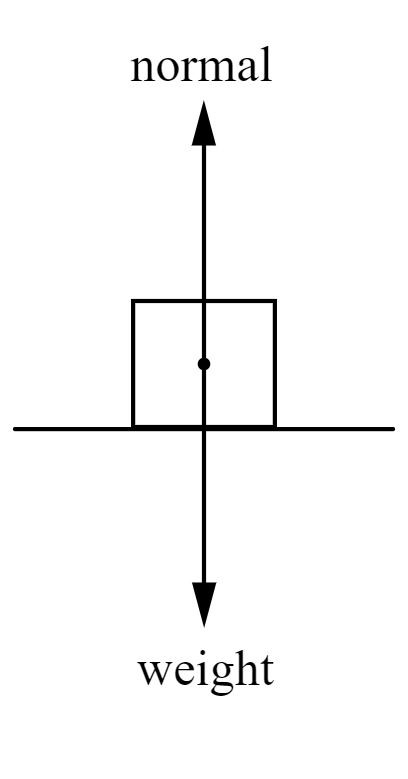
\includegraphics[scale=0.75]{notes/images/Free-Body-Diagram-Book.JPG}
    \caption{A free body diagram of a book lying on a table}
    \label{fig:free-body-diagram-book}
\end{figure}
\FloatBarrier

\subsection{Statics}

Informally, statics is the study of forces without motion. More formally, statics is the branch of mechanics that deals with forces in the absence of changes in motion. In contrast, dynamics is the study of forces and motion; or more formally, the branch of mechanics that deals with the effect that forces have on the motion of bodies. Statics implies stasis. Dynamics implies change (acceleration). 

Statics seems to imply being stationary, but it is not the case; it is merely the absence of acceleration that distinguishes statics from dynamics. When an object doesn't accelerate, it has no resultant force acting on it. This is a consequence of Newton's first law of motion. There are several ways of describing such a situation:
\begin{itemize}
    \item The resultant force is zero.
    \item The forces are balanced.
    \item The system is in equilibrium.
\end{itemize}
The ``resultant force is zero'' relates back to the first law. The resultant force, sometimes referred to as the \textit{net force}, relates to the vector sum of all the separate forces acting on the object. This can be written as $\sum \vec{F}$ or $\vec{F}$. So in a ``statics'' situation $\vec{F} = \vec{0}$.

The ``forces are balanced'' is usually used in situations such as a book on a table, the weight is balanced by the normal contact force from the table. Weight and normal in this case are said to be a pair of balanced forces because one is equal and opposite to the other (note that this is a action-reaction pair of forces in this scenario). If we have a pair of balanced forces, their vector sum is zero. If all the forces on an object are balanced, then we can safely say the forces acting on an object are balanced if and only if the resultant force is zero. Hence providing the equivalence between to first and second statements. We will not discuss the third statement, as we have already mentioned it in passing in other sections (see section \ref{subsection:forces}).  


\subsection{Friction}

As stated in section \ref{subsection:forces}. Friction refers to any force that resists relative tangential motion (or intended motion), whose direction is opposite to the relative direction of motion (or intended motion). ``Relative tangential motion'' is a fancy way to say slipping or sliding. 

There are several types of friction. Although we will only discuss dry and viscous friction in this course. Dry friction ($\vec{F}_f$) is the resistive force between solid surfaces in contact that resist their relative tangential motion, whereas, viscous friction is the resistive force between surfaces in relative motion through a fluid. For example, drag is a type of viscous friction. Viscous friction is dealt with in a different section, see \ref{subsection:drag}. There are a number of factors affecting dry friction:
\begin{itemize}
    \item The magnitude of dry friction $\| \vec{F}_f \|$ is directly proportional to the magnitude of normal contact force $\| \vec{R} \|$ between the two surfaces in contact.
    \item The magnitude of dry friction $\| \vec{F}_f \|$ depends on the materials in contact. This factor is measured by the quantity known as the \textit{coefficient of friction} $\mu$ which exists in the range $0 \leq \mu \leq 1$. Hence the magnitude of dry friction is directly proportional to the coefficient of friction.
\end{itemize}

\noindent We typically divide dry friction into two distinct types: static friction and kinetic friction. 

\begin{itemize}
    \item \textbf{Static friction} ($\vec{F}_{f, s}$) \\
    Static friction, also known as \textit{starting friction}, occurs when the two surfaces in contact \textit{are not} in relative motion; that is, when one surface is stationary relative to the other surface. The magnitude of static frictions varies from zero (when no external force is trying to force slippage) to some maximum value (just before slippage occurs). This maximum value can be determined using the inequality stated below.
    \begin{equation}
        \| \vec{F}_{f, s} \| \leq \mu_s \| \vec{R} \|,
    \end{equation}
    where $\mu_s$ denotes the coefficient of static friction.
    \item \textbf{Kinetic friction} ($\vec{F}_{f, k}$) \\
    Kinetic friction, also known as \textit{sliding} or \textit{dynamic} friction, occurs when two surfaces in contact \textit{are} in relative motion; that is when one surface is slipping or sliding across another surface. The magnitude of kinetic friction varies in a similar fashion to static friction and is always less than the maximum magnitude of static friction. So we have the following relationship;
    \begin{equation}
        \| \vec{F}_{f, k} \| = \mu_k \| \vec{R} \| < \mu_s \| \vec{R} \|,
    \end{equation}
    where $\mu_k$ denotes the coefficient of kinetic friction.
    
    
\end{itemize}


\section{Energy}

\subsection{Work}

If a force is applied to a body, which then moves, we say the force does \textbf{work}. In one-dimension, if the force is \textit{constant} with magnitude $F$, and the body moves a distance $x$, the work done $W$ is 
\begin{equation}
    W = Fx
\end{equation}

\begin{definition}{(\textbf{Work})}
\label{def:work}
\textit{The work done, W, is defined as the product of the magnitude of the force parallel to the direction of motion, $F_{\|}$, and the distance moved $x$ in the direction of motion}
\begin{equation}
    W = F_{\|} x
\end{equation}
\textit{measured in \textbf{joules} (J).}
\end{definition}

\begin{definition}{(\textbf{Joule})}
\textit{A joule is the work done by a force of 1 newton moving through a distance of 1 metre, thus }
\begin{equation*}
    [J] = [Nm] = [kgm^2s^{-2}]
\end{equation*}
\end{definition}

However, the definition of work done (see definition \ref{def:work}) only applies to a one-dimensional model and when the force is applied in the direction of motion. In two-dimensions, the force applied can be at an angle to the direction. The component of the force $\vec{F}$ that is parallel to the direction of motion is $\| \vec{F} \| \cos \theta$, where $\theta$ is the angle between the force and the direction of motion. So, in two-dimensions work done, $W$, is defined as
\begin{equation}
    W = \| \vec{F} \| x\cos \theta
\end{equation}

If we consider the individual dimensions of a multidimensional model and calculated the work done in all dimensions. Summing these produces the total work done. Hence we can consider the dot product of force and displacement to calculate the work done in a multidimensional model.

\begin{definition}{(\textbf{Work})}
\textit{The work done, W, is defined as the \textbf{dot product} of the constant force applied to an object $\vec{F}$ that moves a displacement $\vec{s}$}
\begin{equation}
    W = \vec{F} \cdot \vec{s} 
\end{equation}
\textit{measured in \textbf{joules} (J).}
\end{definition}

If the force is not \textit{constant}, then we must consider a small amount of work done $\mathop{\mathrm{d}W}$ with a force  $\vec{F}$ that moves an object a small displacement $\mathop{\mathrm{d}\vec{s}}$
\begin{equation*}
    \mathop{\mathrm{d}W} = \vec{F} \cdot \mathop{\mathrm{d}\vec{s}} = \vec{F} \cdot \vec{v} \mathop{\mathrm{d}t}
\end{equation*}
which forms a first order differential equation
\begin{equation*}
    \frac{\mathop{\mathrm{d}W}}{\mathop{\mathrm{d}t}} = \vec{F} \cdot \vec{v}
\end{equation*}
and can be solved using
\begin{equation}
    \label{eq:work-done-variable-force-vector}
    W = \int_{t_1}^{t_2} \vec{F} \cdot \vec{v} \mathop{\mathrm{d}t} = \int_{t_1}^{t_2} \vec{F} \cdot \frac{\mathop{\mathrm{d}\vec{s}}}{\mathop{\mathrm{d}t}} \mathop{\mathrm{d}t} = \int_C \vec{F} \cdot \mathop{\mathrm{d}\vec{s}}.
\end{equation}

\subsection{Power}
\label{subsection:power}

\begin{definition}{(\textbf{Power})}
\label{def:power}
\textit{Power, P, is defined as the rate of work done, so}
\begin{equation}
    P = \frac{\mathop{\mathrm{d}W}}{\mathop{\mathrm{d}t}}
\end{equation}
\textit{measured in \textbf{watts} (W)}
\end{definition}

\begin{corollary}
\textit{It follows, that if the force $\vec{F}$ is constant then power $P$ is}
\begin{equation}
    P = \vec{F} \cdot \vec{v}
\end{equation}
\textit{where $\vec{v}$ is velocity.}

\begin{proof}
\textit{By definition of power we have}
\begin{equation*}
    P = \frac{\mathop{\mathrm{d}W}}{\mathop{\mathrm{d}t}}
\end{equation*}
\textit{If the force $\vec{F}$ is constant, by definition we have}
\begin{equation*}
    \mathop{\mathrm{d}W} = \vec{F} \cdot \mathop{\mathrm{d}\vec{s}}
\end{equation*}
\textit{then,}
\begin{equation*}
    P = \vec{F} \cdot \frac{\mathop{\mathrm{d}\vec{s}}}{\mathop{\mathrm{d}t}} = \vec{F} \cdot \vec{v}.
\end{equation*}
\end{proof}
\end{corollary}

\subsection{Energy}
\label{subsection:energy}
If a body has the capacity (or ability) to do work, we say it has \textbf{energy}.
\begin{definition}{(\textbf{Energy})}
\textit{Energy is defined as the capacity for doing work, which implies, the energy of the body is amount of work it can do. Measured in \textbf{joules} (J).}
\end{definition}

When the body does some work it uses some of it's energy, but if work is done on the body then it's energy increases. Energy comes in many forms (thermal, electrical, \ldots) but we consider only \textit{mechanical energy} (in section \ref{subsection:energy}). Mechanical energy is of two types;
\begin{enumerate}
    \item \textit{kinetic energy} - the ability to do work by virtue of velocity.
    \item \textit{potential energy} - ability to do work by virtue of position in a gravitational field.
\end{enumerate}

\subsection{Equivalence of Work and Energy}

When work is done on a body by applying a force which moves through a distance, then it's energy increases by the amount of work done.
Similarly, a body which possesses energy, either kinetic or potential, can give up that energy by doing work. Hence we say \textbf{Work and Energy are equivalent} and are both measured in \textit{\textbf{Joules} (J)}.

\subsection{Conservation of Energy}

If no work is done on or by a body, then body is said to be in a \textbf{closed system}. We say:

\begin{center}
    \textit{The total energy of a closed system remains constant. The energy can never be created or destroyed, but it can be transferred from one from to another.}
\end{center}

\noindent This is called the \textbf{Principle of conservation of energy}.

\subsection{Kinetic Energy}

\begin{definition}{(\textbf{Kinetic Energy})}
\textit{The kinetic energy of a body, $E_k$, with a mass $m$ and velocity $v$ is given by}
\begin{equation}
    E_k = \frac{1}{2}m \| \vec{v} \|^2
\end{equation}
\textit{measured in \textbf{joules} (J).}
\begin{proof}
\textit{Consider a particle of mass $m$ that is accelerated from rest to velocity $\vec{v}$ in a distance $\| \vec{s} \|$ by a constant force $\vec{F}$. From the equation of motion $\| \vec{v} \|^2 = \| \vec{u} \|^2 + 2\vec{a} \cdot \vec{s}$ and Newton's II law of motion, we have}
\begin{equation*}
    \| \vec{v} \|^2 = \frac{2}{m} \vec{F} \cdot \vec{s}
\end{equation*}
\begin{equation*}
    \vec{F} \cdot \vec{s} = \frac{1}{2}m\| \vec{v} \|^2
\end{equation*}
\textit{The work done by the force is entirely transferred to the Kinetic energy of the particle. Therefore}
\begin{equation*}
    W = E_k = \vec{F} \cdot \vec{s}
\end{equation*}
\textit{Hence}
\begin{equation*}
    E_k = \frac{1}{2}m \| \vec{v} \|^2
\end{equation*}
\end{proof}
\end{definition}

\subsection{Potential Energy}

\textbf{Potential energy}, also referred to as \textbf{gravitational potential energy}, is the capacity for doing work as a result of an object's position in a gravitational field.

\begin{definition}{(\textbf{Potential Energy})}
\textit{The potential energy of a body, $E_p$, with mass $m$ and change in height $h$ in a \textbf{uniform gravitational field} with gravitational field strength $\| \vec{g} \|$ is}
\begin{equation}
    E_p = m\| \vec{g} \|h
\end{equation}
\end{definition}

\begin{corollary}
\textit{In many situations, potential energy and kinetic energy are exchanged. For example, when an object falls its $E_p$ decreases while its $E_k$ increases. It follows from the \textbf{principle of conservation of energy}, that the lost in $E_p$ is equal to the gain in $E_k$}
\begin{align*}
    m\| \vec{g} \|h &= \frac{1}{2}m\| \vec{v} \|^2 \\
    \| \vec{g} \|h &= \frac{1}{2} \| \vec{v} \|^2 \\
    \| \vec{v} \|^2 &= 2\| \vec{g} \|h \\
    \| \vec{v} \| &= \sqrt{2\| \vec{g} \|h}
\end{align*}
\textit{provided the system is closed and the change in height $h > 0$}.
\end{corollary}

\section{Dynamics II: Momentum}

\subsection{Impulse and Momentum}
\label{subsection:impulse-and-momentum}

Momentum keeps me going. It is a ``quantity of motion'' (from \textit{Principa}). Almost a resistance to stopping. 

\begin{definition}{(\textbf{Momentum})}
\textit{Momentum is the product of the mass and velocity of an object. Mathematically, }
\begin{equation}
    \vec{p} = m \vec{v},
\end{equation}
\textit{where $\vec{p}$ is the momentum of the object (a vector quantity), m is the object's mass and $\vec{v}$ is the velocity. It is measured in \textbf{kilogram meters per second} ($kgms^{-1}$)}
\end{definition}

We know from Newton's second law of motion, that the resultant force is directly proportional to the rate of change of momentum. 
\begin{equation*}
    \vec{F} = \frac{\mathop{\mathrm{d}\vec{p}}}{\mathop{\mathrm{d}t}}.
\end{equation*}
Separating the variables, we have
\begin{equation*}
    \vec{F} \mathop{\mathrm{d}t} = \mathop{\mathrm{d}\vec{p}},
\end{equation*}
integrating both sides yields a new quantity. We'll call it \textbf{impulse}, denoted by the letter $\vec{J}$. Thus,
\begin{equation}
    \label{eq:impulse-momentum-theorem}
    \vec{J} = \int_{\vec{p}_0}^{\vec{p}_1} \mathop{\mathrm{d}\vec{p}} = \int_0^t \vec{F} \mathop{\mathrm{d}t}
\end{equation}
Impulse is measured in \textit{newton seconds} or \textit{kilogram meters per second} which is dimensionally equivalent to momentum. This relationship is called the \textbf{impulse-momentum theorem}, which states that \textit{impulse causes a change in momentum}. Evaluating the first integral in equation \ref{eq:impulse-momentum-theorem} give us
\begin{equation}
    \vec{J} = \vec{p}_1 - \vec{p}_0 = \Delta \vec{p} = \int_0^t \vec{F} \mathop{\mathrm{d}t}.
\end{equation}

\subsection{Conservation of Momentum}

Suppose that two particles interact labelled one and two respectively. Because of the third law of motion, the forces between them are equal and opposite, so we have
\begin{equation}
    \vec{F}_{1,2} = - \vec{F}_{2,1}.
\end{equation}
The second law states that
\begin{equation}
    \vec{F}_{1,2} = \frac{\mathop{\mathrm{d}\vec{p}_1}}{\mathop{\mathrm{d}t}} \text{ and } \vec{F}_{2,1} = \frac{\mathop{\mathrm{d}\vec{p}_2}}{\mathop{\mathrm{d}t}}.
\end{equation}
Therefore,
\begin{equation}
    \frac{\mathop{\mathrm{d}}}{\mathop{\mathrm{d}t}} (\vec{p}_1 + \vec{p}_2) = \vec{0},
\end{equation}
implying that $\vec{p}_1 + \vec{p}_2$ is constant over time. So in a closed system the total momentum is constant. Hence we can say
\begin{align}
    \vec{p}_1 + \vec{p}_2 &= \vec{p}_1^{'} + \vec{p}_2^{'} \\
    \sum \vec{p} &= \sum \vec{p}'
\end{align}

\subsection{Collisions}

The conservation of momentum, discussed in the previous section, can be applied to collisions to determine the motion of particles after a collision. Another property of motion, kinetic energy, is also required to determine the motion of particles after collision. However, this is not necessarily conserved. If it is conserved, the collision is called an \textit{elastic} collision; if not, it is an \textit{inelastic collision}.  

If we consider an elastic collision between two particles, then by the conservation of momentum we have
\begin{equation}
    \vec{p}_1 + \vec{p}_2 = \vec{p}_1^{'} + \vec{p}_2^{'}.
\end{equation}
Let particle one have a mass of $m_1$ kg and an initial and final velocity of $\vec{u}_1$ and $\vec{v}_1$ respectively. Similarly for particle two, we apply the same labelling scheme. So from the definition of momentum, it follows that
\begin{equation}
    m_1 \vec{u}_1 + m_2 \vec{u}_2 = m_1 \vec{v}_1 + m_2 \vec{v}_2.
\end{equation}
If the both masses and three of the velocities are known, then it is possible to determine the unknown velocity.

\section{Rotational Motion}

\subsection{Motion in Plane Polar Coordinates}

A particle of mass $m$ may have a position $\vec{r}$ defined by a column vector, that is $\vec{r} = \langle r_1, r_2, \ldots, r_n \rangle$ or a \textbf{polar vector} with a magnitude $r$ and a direction $\theta$ such that $\vec{r} = \langle r, \theta \rangle$. Let us introduce a unit radial vector $\hat{r}$ and a unit transverse vector $\hat{\theta}$; where $\hat{r}$ and $\hat{\theta}$ are orthogonal (perpendicular) to each other. The position vector $\vec{r}$ is now given by $\vec{r} = r \hat{r}$. For example, in a two dimensional model the unit radial and transverse vectors are given by
\begin{align*}
    \hat{r} &= \langle \cos \theta, \sin \theta \rangle \\
    \hat{\theta} &= \langle - \sin \theta, \cos \theta \rangle
\end{align*}
As the particle moves in a two dimensional model, the magnitude $r$ and directions of $\hat{r}$ and $\hat{\theta}$ vary, implying they're functions of time. If we now consider the velocity of the particle, we find
\begin{equation}
    \vec{v} = \frac{\mathop{\mathrm{d} \vec{r}}}{\mathop{\mathrm{d} t}} = \frac{\mathop{\mathrm{d}}}{\mathop{\mathrm{d}t}}(r \hat{r}) = \frac{\mathop{\mathrm{d}r}}{\mathop{\mathrm{d} t}} \hat{r} + r \frac{\mathop{\mathrm{d} \hat{r}}}{\mathop{\mathrm{d} t}}
\end{equation}
An expression for $\frac{\mathop{\mathrm{d} \hat{r}}}{\mathop{\mathrm{d} t}}$ can be found by considering the expression for the unit radial vector (shown above), so we have
\begin{align*}
    \hat{r} &= \langle \cos \theta, \sin \theta \rangle \\
    \frac{\mathop{\mathrm{d} \hat{r}}}{\mathop{\mathrm{d} t}} &= \left\langle - \sin \theta \frac{\mathop{\mathrm{d} \theta}}{\mathop{\mathrm{d}t}}, \cos \theta \frac{\mathop{\mathrm{d} \theta}}{\mathop{\mathrm{d} t}}\right\rangle \\
    &= \frac{\mathop{\mathrm{d} \theta}}{\mathop{\mathrm{d}t}} \langle -\sin \theta, \cos \theta \rangle \\
    &= \frac{\mathop{\mathrm{d} \theta}}{\mathop{\mathrm{d}t}} \hat{\theta},
\end{align*}
So 
\begin{equation}
    \vec{v} = \frac{\mathop{\mathrm{d}r}}{\mathop{\mathrm{d} t}} \hat{r} + r \frac{\mathop{\mathrm{d} \theta}}{\mathop{\mathrm{d} t}} \hat{\theta}
\end{equation}
We say the radial component of $\vec{v}$ is $\frac{\mathop{\mathrm{d}r}}{\mathop{\mathrm{d} t}}$ and the transverse component is $r \frac{\mathop{\mathrm{d} \theta}}{\mathop{\mathrm{d} t}}$. An often used abbreviation for differentiation with respect to time is to put a ``dot'' above the quantity, so for the above expression for $\vec{v}$ is written as
\begin{equation}
    \vec{v} = \dot{\vec{r}} = \dot{r} \hat{r} + r \dot{\theta} \hat{\theta}
\end{equation}
The instantaneous speed of the particle  is given by
\begin{equation}
    \label{eq:polar-speed}
    v = \| \vec{v} \| = \sqrt{\vec{v} \cdot \vec{v}} = \sqrt{\left(\frac{\mathop{\mathrm{d}r}}{\mathop{\mathrm{d} t}}\right)^2 + r^2 \left(\frac{\mathop{\mathrm{d} \theta}}{\mathop{\mathrm{d} t}}\right)^2} = \sqrt{\dot{r}^2 + r^2 \dot{\theta}^2}.
\end{equation}
We now consider the acceleration of the particle, applying the product rule again to give
\begin{align*}
    \vec{a} &= \frac{\mathop{\mathrm{d}\vec{v}}}{\mathop{\mathrm{d}t}} = \frac{\mathrm{d}}{\mathop{\mathrm{dt}}} \left(\frac{\mathop{\mathrm{d}r}}{\mathop{\mathrm{d} t}} \hat{r} + r \frac{\mathop{\mathrm{d} \theta}}{\mathop{\mathrm{d} t}} \hat{\theta}\right) \\
    &= \frac{\mathop{\mathrm{d}^2 r}}{\mathop{\mathrm{dt^2}}} \hat{r} + \frac{\mathop{\mathrm{d}r}}{\mathop{\mathrm{d}t}} + 2 \frac{\mathop{\mathrm{d}r}}{\mathop{\mathrm{d}t}}\frac{\mathop{\mathrm{d}\theta}}{\mathop{\mathrm{d}t}} \hat{\theta} + r \hat{\theta} \frac{\mathop{\mathrm{d}^2 \theta}}{\mathop{\mathrm{d}t^2}} + r \frac{\mathop{\mathrm{d}\theta}}{\mathop{\mathrm{d}t}} \frac{\mathop{\mathrm{d}\hat{\theta}}}{\mathop{\mathrm{d}t}}
\end{align*}
Using the same method we used to find $\ddot{\hat{r}}$, we find that
\begin{equation*}
    \frac{\mathop{\mathrm{d} \hat{\theta}}}{\mathop{\mathrm{d} t}} = - \frac{\mathop{\mathrm{d} \theta}}{\mathop{\mathrm{d} t}} \hat{r},
\end{equation*}
so we have
\begin{align}
    \vec{a} &= \left(\frac{\mathop{\mathrm{d}^2 r}}{\mathop{\mathrm{d}t^2}} - r \left(\frac{\mathop{\mathrm{d}\theta}}{\mathop{\mathrm{d}t}}\right)^2 \right) \hat{r} + \left(2 \frac{\mathop{\mathrm{d}r}}{\mathop{\mathrm{d}t}} \frac{\mathop{\mathrm{d}\theta}}{\mathop{\mathrm{d}t}} + r \frac{\mathop{\mathrm{d}^2 \theta}}{\mathop{\mathrm{d}t^2}}\right) \hat{\theta} \\
    &= \left(\ddot{r} - r \dot{\theta}^2 \right) \hat{r} + \left(2 \dot{r} \dot{\theta} + r \ddot{\theta}\right) \hat{\theta}
\end{align}
So the radial component of acceleration is $\ddot{r} - r \dot{\theta}^2$ and the transverse component is $2 \dot{r} \dot{\theta} + r \ddot{\theta}$.

\subsection{Circular Motion}

Consider a particle moving in a circle with a radius $r$ as shown in figure \ref{fig:circular-motion}. Then $r$ is constant, so $\dot{r} = 0$ and $\ddot{r} = 0$, hence
\begin{equation}
    \vec{v} = r \dot{\theta} \hat{\theta},
\end{equation}
so the velocity is purely transverse. 

\begin{figure}[h!]
    \centering
    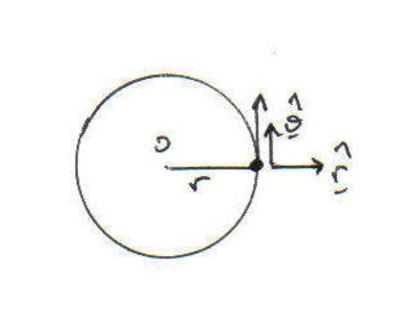
\includegraphics[scale=0.6]{notes/images/Circular-Motion.JPG}
    \caption{Motion in a circle}
    \label{fig:circular-motion}
\end{figure}
\FloatBarrier

From the definition of velocity, it also follows that the displacement $\vec{s}$ of the particle is given by
\begin{equation}
    \vec{s} = r \theta \hat{\theta}.
\end{equation}
We sometimes write the \textbf{angular velocity} as $\omega = \frac{\mathop{\mathrm{d}\theta}}{\mathop{\mathrm{d}t}} = \dot{\theta}$ which is measured in \textbf{radians per second} ($\text{rad} s^{-1}$), although revolutions per minute ($\text{rpm}$) is occasionally used, in which case
\begin{equation}
    \vec{v} = r \omega \hat{\theta}.
\end{equation}
The acceleration of the particle is given by
\begin{equation}
    \vec{a} = \left( -r\dot{\theta}^2\right) \hat{r} + r \ddot{\theta} \hat{\theta}.
\end{equation}
If the angular velocity is constant, it implies $\dot{\omega} = \ddot{\theta} = 0$, and 
\begin{equation}
    \vec{a} = -r \dot{\theta}^2 \hat{r} = -r \omega^2 \hat{r}.
\end{equation}
and the acceleration is directed towards the centre of the circle, since we only have the radial component $- r \omega^2$. Since $\vec{v} = r \omega \hat{\theta}$ with a magnitude of $\| \vec{v} \| = r \omega$ and so
\begin{equation}
    \vec{a} = - \frac{\| \vec{v} \|^2}{r} \hat{r}.
\end{equation}
This acceleration is called the \textbf{centripetal acceleration}. It follows from Newton's second law of motion that there \textit{must} exist a force $\vec{F}$, such that
\begin{equation}
    \vec{F} = m \vec{a} = - m r \omega^2 \hat{r} = - m \frac{\| \vec{v} \|^2}{r} \hat{r},
\end{equation}
which also acts radially, towards the centre of the circle and has the radial component of $- m r \omega^2$ or $- m \frac{\| \vec{v} \|^2}{r}$.

\subsection{Central forces}
\label{subsection:central-forces}
A \textbf{central force} is one which is purely radial (directed along a radius), either towards or away from the centre, such that
\begin{equation}
    \vec{F}(r) = F(r) \hat{r}.
\end{equation}
If $F(r)$ is positive, the force is said to be \textbf{repulsive} or \textbf{centrifugal}; whereas if $F(r)$ is negative the force is \textbf{attractive} or \textbf{centripetal}. 

Applying Newton's second law of motion and acceleration in plane polar coordinates yields the following equations of motion
\begin{equation}
    m\left[\left(\ddot{r} - r \dot{\theta}^2\right)\hat{r} + \left(2 \dot{r} \dot{\theta} + r \ddot{\theta}\right)\hat{\theta}\right] = F(r)\hat{r}
\end{equation}
We see that the force is entirely radial, so
\begin{align}
    m\left(\ddot{r} - r\dot{\theta}^2\right) &= F(r) \\
    m(2\dot{r}\dot{\theta} + r\ddot{\theta}) &= 0
\end{align}
We define the \textbf{magnitude} of \textbf{angular momentum}, $\| \vec{L} \|$ of a particle about a point $O$ as
\begin{equation}
    \| \vec{L} \| = mr \| \vec{v}_{\theta} \| = mr^2 \dot{\theta},
\end{equation}
where $\vec{v}_{\theta}$ is the transverse component of velocity in plane polar coordinates. Thus
\begin{align}
    \frac{\mathop{\mathrm{d}\| \vec{L} \|}}{\mathop{\mathrm{d}t}} &= m\left(2 r \dot{r} \dot{\theta} + r^2 \ddot{\theta}\right) \\
    &= mr\left(2\dot{r}\dot{\theta} + r \ddot{\theta}\right) \\
    &= mr\| \vec{a}_{\theta} \|,
\end{align}
where we denote the transverse acceleration as $\vec{a}_{\theta} = \left(2\dot{r}\dot{\theta} + r \ddot{\theta}\right) \hat{\theta}$. However, for a central force, the transverse acceleration is zero, so
\begin{equation}
    \frac{\mathop{\mathrm{d}\| \vec{L} \|}}{\mathop{\mathrm{d}t}} = 0,
\end{equation}
and hence the magnitude angular momentum $\| \vec{L} \|$ is constant during the motion of any central force.

\subsection{Rotating Frame of Reference}

Consider an observer $A$ standing on a rotating disk as shown in figure ??. 

The real force of friction at the feet provides the centripetal acceleration $-r\omega^2 \hat{r}$, therefore $\vec{F} = -mr\omega^2\hat{r}$. \textbf{Relative to the disk} the person is at \textbf{rest} under the influence of a real centripetal force and a \textbf{fictitious} \textbf{\textit{centrifugal force}} (\textit{yes, its exists!}) $\mathfrak{F}_{cent} = mr\omega^2\hat{r}$ acting through the centre of mass. 

\begin{example}{(\textbf{A Geostationary Satellite})}
Consider a geostationary satellite, a satellite that appears stationary relative to an observer on a rotating Earth as shown below.

The real force on the satellite is the gravitational force (centripetal force);
\begin{equation*}
    \vec{F} = - mr \omega^2 \hat{r}.
\end{equation*}
The observer on Earth thinks there is also a fictitious centrifugal force (by Newton's first law of motion),
\begin{equation*}
    \mathfrak{F}_{cent} = mr \omega^2 \hat{r}
\end{equation*}
so there is no resultant force, and so the satellite is at rest and in equilibrium with respect to this frame.
\end{example}

We discussed the relative positions of moving points in inertial reference frames in section ??, we will do the same for rotating frames of reference. Consider an observed $B$ at rest on a spinning disk observing a moving body, e.g. a flying bird, as shown in figure ??. Consider the same bird being observed by a second observer $A$ at rest relative to the Earth. The path of the bird, as observed by $A$, is a straight line, however, relative to observer $B$ the path of the bird is curved. So observer $B$ can assume there is a transverse horizontal force $\mathfrak{F}_{cor}$ acting on the bird, deflecting the bird to the right for the given sense of rotation. This is known as the \textbf{Coriolis force}, whose magnitude is given by
\begin{equation}
    \mathfrak{F}_{cor}  = - 2 m \dot{r} \omega \hat{\theta},
\end{equation}
where $\omega$ is the angular velocity of the rotating frame, $\dot{r}$ is the radial velocity and $m$ is the mass of the particle.

To find the Coriolis force, let us consider a massless smooth rod on which there is a disk of mass $m$. The rod is rotating with a constant angular velocity $\omega$ in a horizontal plane. As the rood is smooth there can be no radial force (from friction) on the pivot of the disk. The only force on the pivot is a transverse normal reaction force $\vec{F}_n$ as shown in the figure below. 


The equation of motion of the pivot is (relative to the inertial reference frame),
\begin{equation}
    m \vec{a} = \vec{F}_n
\end{equation}
\begin{equation}
    m \left[ \left(\ddot{r} - r \dot{\theta}^2 \right) \hat{r} + \left(2 \dot{r} \dot{\theta} + r \ddot{\theta}\right) \hat{\theta} \right] = \| \vec{F}_n \| \hat{\theta}
\end{equation}
Therefore the radial equation of motion is
\begin{equation}
    m \left(\ddot{r} - r \dot{\theta}^2 \right) \hat{r} = \vec{0}
\end{equation}
and the transverse one is
\begin{equation}
    m \left(2 \dot{r} \dot{\theta} + r \ddot{\theta} \right) \hat{\theta} = \| \vec{F}_n \| \hat{\theta}.
\end{equation}
But, we have a constant angular velocity, so $\ddot{\theta} = \dot{\omega} = 0$, giving us
\begin{equation}
    m \left(\ddot{r} - r \omega^2 \right) \hat{r} = \vec{0} 
\end{equation}
and
\begin{equation}
    2 m \dot{r} \omega \hat{\theta} = \| \vec{F}_n \| \hat{\theta}
\end{equation}

Now consider the equations of motion of the pivot relative to the rotating rod. In this frame the pivot can only move in on dimension along the rod. if we work in this frame we must add fictitious forces to the real forces, such as the fictitious centrifugal force $\mathfrak{F}_{cent}$ and the Coriolis force $\mathfrak{F}_{cor}$; as shown in figure ??

In the rotating frame the radial equation of motion is
\begin{equation}
    m \ddot{r} \hat{r} = \mathfrak{F}_{cent}
\end{equation}
and for the transverse component, we have
\begin{equation}
    \vec{F}_n + \mathfrak{F}_{cor} = \vec{0},
\end{equation}
as there is no transverse motion in the rotating frame. We can now compare the radial and transverse equations of motion in each frame to find the fictitious centrifugal and Coriolis forces. Comparing equation ?? with equation ?? gives the centrifugal force
\begin{equation}
    \mathfrak{F}_{cent} = m r \omega^2 \hat{r}
\end{equation}
and comparing equations ?? and ?? gives the Coriolis force
\begin{equation}
    \mathfrak{F}_{cor} = -2m\dot{r}\omega \hat{\theta}
\end{equation}

Despite this argument being mathematically valid, it isn't valid for 3 dimensions. In order to find the Coriolis force in 3 dimensions, we need to consider a pseudo surface-vector for angular velocity with respect to plane of rotation

\subsection{Torque}

\textbf{Torque} or \textbf{moments} are the rotational equivalent of linear force. Just as force can be thought as a push or a pull, a torque can be thought of as a twist to an object. We typically denote torque using $\vec{\tau}$. When referring to a moment of a force, it is more commonly denoted by $M$.

In three dimensions, the torque is a \textit{pseudo-vector}. It is given by the cross product of the radial vector and the force vector. So we have
\begin{equation}
    \vec{\tau} = \vec{r} \times \vec{F},
\end{equation}
where the magnitude is given by
\begin{equation}
    \| \vec{\tau}\| = \|\vec{r}\|\| \vec{F}\|\sin \theta,
\end{equation}
where $\theta$ is the angle between the force vector and the radial vector. The SI unit for torque is the \textbf{Newton metre} ($Nm$). The direction of torque is determined by the right-hand rule.

The unbalanced torque on a body along the axis of rotation determines the rate of change of the body's angular momentum. 

\begin{equation}
     \vec{\tau}  = \frac{\mathop{\mathrm{d} \vec{L} }}{\mathop{\mathrm{d}t}}.
\end{equation}

If multiple torques are acting on the body, it is instead the net torque which determines the rate of change of the angular momentum

\begin{equation}
    \vec{\tau}_1 + \cdots + \vec{\tau}_n = \vec{\tau}_{net}  = \frac{\mathop{\mathrm{d} \vec{L}}}{\mathop{\mathrm{d}t}}.
\end{equation}

The equivalence of angular momentum and torque can be proved easily by considering the following definition of angular momentum $\vec{L}$: 
\begin{equation}
    \vec{L} = \vec{r} \times \vec{p},
\end{equation}
where $\vec{r}$ is the radial vector and $\vec{p}$ is the particle's linear momentum. So the time derivative of this is
\begin{equation}
    \frac{\mathop{\mathrm{d}\vec{L}}}{\mathop{\mathrm{d}t}} = \vec{r} \times \frac{\mathop{\mathrm{d}\vec{p}}}{\mathop{\mathrm{d}t}} + \frac{\mathop{\mathrm{d}\vec{r}}}{\mathop{\mathrm{d}t}} \times \vec{p}
\end{equation}
From Newton's second law of motion we have $\vec{F} = \frac{\mathop{\mathrm{d}\vec{p}}}{\mathop{\mathrm{d}t}}$ and the definition of velocity (in rotational motion) is $\vec{v} = \frac{\mathop{\mathrm{d}\vec{r}}}{\mathop{\mathrm{d}t}}$. So
\begin{equation}
    \frac{\mathop{\mathrm{d}\vec{L}}}{\mathop{\mathrm{d}t}} = \vec{r} \times \vec{F} + \vec{v} \times \vec{p}
\end{equation}
The cross product of linear momentum $\vec{p}$ and velocity $\vec{v}$ is zero because velocity and momentum are parallel. So it follows that
\begin{equation}
    \frac{\mathop{\mathrm{d}\vec{L}}}{\mathop{\mathrm{d}t}} = \vec{r} \times \vec{F}_{net} = \vec{\tau}_{net}
\end{equation}

\subsubsection*{Rotational Work}
If a force acts through a distance, it is doing work. Similarly, if torque acts through a rotational distance, it is doing work. Mathematically, for rotation about a fixed axis through the centre of mass,
\begin{equation}
    W = \int_{\theta_1}^{\theta_2} \| \vec{\tau} \| \mathop{\mathrm{d}\theta}.
\end{equation}
Let us consider the definition of work done,
\begin{equation}
    W = \int_C \vec{F} \cdot \mathop{\mathrm{d}\vec{s}}
\end{equation}
However, for an infinitesimal displacement $\mathop{\mathrm{d}\vec{s}}$ is related to a corresponding angular displacement $\mathop{\mathrm{d}\vec{\theta}}$ and the radial vector $\vec{r}$ as
\begin{equation}
    \mathop{\mathrm{d}\vec{s}} = \mathop{\mathrm{d}\vec{\theta}} \times \vec{r}
\end{equation}
Substituting this into equation ?? yields
\begin{equation}
    W = \int_{\vec{\theta}_1}^{\vec{\theta}_2} \vec{F} \cdot (\mathop{\mathrm{d}\vec{\theta}} \times \vec{r})
\end{equation}
Notice the triple scalar product in the integrand above, which can be rewritten as
\begin{equation}
    W = \int_{\vec{\theta}_1}^{\vec{\theta}_2} (\vec{r} \times \vec{F}) \cdot \mathop{\mathrm{d}\vec{\theta}}
\end{equation}
From the definition of torque, we have
\begin{equation}
    W = \int_{\vec{\theta}_1}^{\vec{\theta}_2} \vec{\tau} \cdot \mathop{\mathrm{d}\vec{\theta}}
\end{equation}
Given torque and angular displacement are always parallel, then the scalar product simply reduces to a product of magnitudes, so
\begin{equation}
    W = \int_{\theta_1}^{\theta_2} \| \vec{\tau} \| \mathop{\mathrm{d}\theta}.
\end{equation}

\subsubsection*{The Principle of Moments}

The Principle of Moments, simply states that the sum of torques applied to a single point is equal to the torque due to the sum (resultant) of the forces. Mathematically, this is
\begin{equation}
    (\vec{r} \times \vec{F}_1) + (\vec{r} \times \vec{F}_2) + \cdots = \vec{r} \times (\vec{F}_1 + \vec{F}_2 + \cdots)
\end{equation}
A corollary of this is that for a body in rotational equilibrium the sum of the torques acting on the body is zero. 

However, in A2 Physics, we learn \textbf{wrong} Physics, so instead the Principle of Moments states that for a body in rotational equilibrium, the sum of the clockwise moments about any point is equal to the sum of anticlockwise moments about the same point 

\subsubsection*{Couples}

A \textbf{couple} refers to a pair of parallel forces that are equal in magnitude, but oppositely directed. The forces have a turning effect or moment called a torque above an axis which is perpendicular to the plane of the forces. 

FIGURE HERE

If the two forces are $\vec{F}$ and $-\vec{F}$, then the magnitude of the torque is given by
\begin{equation}
    \| \vec{\tau} \| = \| \vec{F} \| d
\end{equation}


\section{Planetary Motion}

\subsection{The Universal Law of Gravitation}

The universal law of gravitation, also know as \textbf{Newton's law of gravitation}, states that the magnitude of the \textbf{gravitational force} $\vec{F}$ between any two particles with masses $m_1$ and $m_2$ is proportional to the product of the two masses and inversely proportional to the square of their separation $r$.
\begin{equation*}
    \| \vec{F} \| \propto \frac{m_1 m_2}{r^2}.
\end{equation*}
The constant of proportionality is denoted as $G$, the \textbf{gravitational constant}. So we say the gravitational force $\vec{F}_{1,2}$ exerted on particle $1$ due to particle $2$ with masses $m_1$ and $m_2$ and position vectors $r_1$ and $r_2$ respectively is 
\begin{equation}
    \vec{F}_{1,2} = - \frac{G m_1 m_2}{\| \vec{r}_{2,1} \|^2} \hat{r}_{2,1}
    \label{eq:gravitational-force}
\end{equation}
and $\vec{r}_{2,1}$ is the separation vector pointing from particle 2 to particle 1, hence
\begin{equation}
    \hat{r}_{2,1} = \frac{\vec{r}_{2,1}}{\| \vec{r}_{2,1} \|} \text{ and } \vec{r}_{2, 1} = \vec{r}_1 - \vec{r}_2.
\end{equation}
We note that by Newton's third law of motion, the force on the particle with $m_2$ exerted by $m_1$ is given by
\begin{equation}
    \vec{F}_{2, 1} = -\vec{F}_{1, 2}.
\end{equation}

The gravitational force is an example of a \textbf{central force} (See section \ref{subsection:central-forces}).

\begin{figure}[h!]
    \centering
    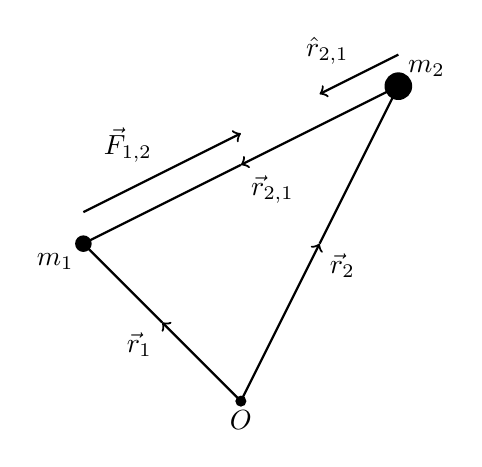
\begin{tikzpicture}
        \coordinate (O) at (0,0);
        \coordinate (A) at (2,4);
        \coordinate (B) at (-2,2);
        
        \fill (O) circle[radius=2pt] node[below] {$O$};
        \fill (A) circle[radius=5pt] node[above right] {$m_2$};
        \fill (B) circle[radius=3pt] node[below left] {$m_1$};
        
        \draw[->, thick] (O) -- (-1,1) node[below left] {$\vec{r}_1$};
        \draw[thick] (-1,1) -- (B);
        \draw[->, thick] (O) -- (1,2) node[below right] {$\vec{r}_2$};
        \draw[thick] (1,2) -- (A);
        
        \draw[->, thick] (-2,2.4) -- (0,3.4) node[midway, above left] {$\vec{F}_{1,2}$};
        \draw[->, thick]  (A) -- (0,3) node[below right] {$\vec{r}_{2,1}$};
        \draw[thick] (0,3) -- (B);
        
        \draw[->, thick] (2,4.4) -- (1,3.9) node[midway, above left] {$\hat{r}_{2,1}$};
    \end{tikzpicture}
    \caption{Vector diagram showing the geometry of the gravitational attraction}
\end{figure}
\FloatBarrier

\subsection{Gravitational Fields}

While two particles are needed to produce a gravitational force, a \textbf{gravitational field} for any single particle in space is used to describe it's effect on other particles. We say a particle $p$ in space produces a gravitation field $\vec{g}$ with spherical symmetry. We have
\begin{equation}
    \label{eq:gravitational-field-1}
    \vec{g} = - \frac{Gm_1}{\| \vec{r} \|^2} \hat{r}
\end{equation}
and so we have
\begin{equation}
    \label{eq:gravitational-field-2}
    \vec{g} = \frac{\vec{F}}{m_2}
\end{equation}
where $\hat{r}$ is a unit surface vector and $\vec{r}$ is a radial vector that is always perpendicular to the surface of the particle. So $\vec{r}$ is always pointing away from the particle towards other particles. In field theory, we represent a gravitational field as a vector field, however, in this course we will use \textit{field lines} to represent the gravitational field.

\begin{figure}[h!]
    \centering
    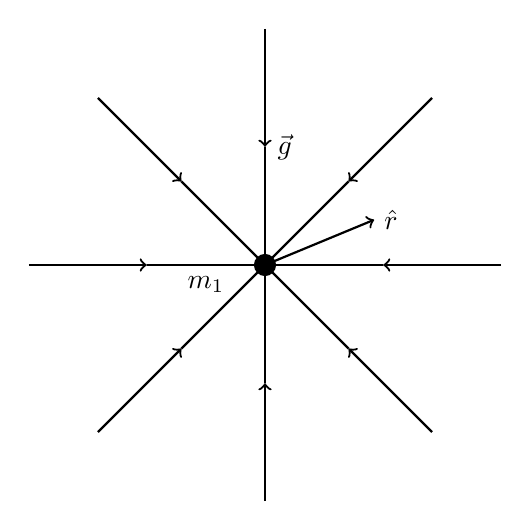
\begin{tikzpicture}
        \coordinate (O) at (0,3);

        
        \fill (O) circle[radius=4pt];
        
        \node at (-0.75,2.75) {$m_1$};
        
        \foreach \i in {1,...,8} {
            \pgfmathsetmacro{\cosValue}{cos(\i * 45)};
            \pgfmathsetmacro{\sinValue}{sin(\i * 45)};
            \draw[->, thick] (3 * \cosValue, 3 * \sinValue + 3) -- (1.5 * \cosValue,1.5 * \sinValue + 3);
            \draw[thick] (1.5 * \cosValue,1.5 * \sinValue + 3) -- (0,3);
        }
        
        \node at (0.25,4.5) {$\vec{g}$};
        \pgfmathsetmacro{\cosValue}{cos(22.5)};
        \pgfmathsetmacro{\sinValue}{sin(22.5)};
        \draw[->, thick] (0,3) -- (1.5 * \cosValue,1.5 * \sinValue + 3) node[at end, right] {$\hat{r}$};
    \end{tikzpicture}
    \caption{Vector diagram showing the geometry of the gravitational field}
\end{figure}
\FloatBarrier

The figure above shows a radial gravitational field of a particle. A \textbf{uniform gravitational field} is said to have field lines that are parallel and equidistant. The field at the surface of the particle is \textit{approximately} uniform. 

\begin{figure}[h!]
    \centering
    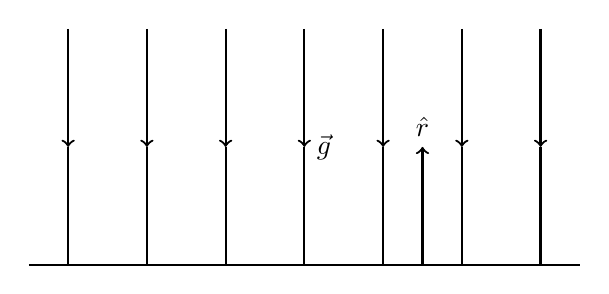
\begin{tikzpicture}
        \draw[thick] (-3.5,0) -- (3.5,0);
        
        \foreach \i in {-3,...,3} {
            \draw[->, thick] (\i,3) -- (\i,1.5);
            \draw[thick] (\i,1.5) -- (\i,0);
        }
        
        \node at (0.25,1.5) {$\vec{g}$};
        \draw[->, thick] (1.5,0) -- (1.5,1.5) node[at end, above] {$\hat{r}$};
    \end{tikzpicture}
    \caption{Vector diagram showing the geometry of a uniform gravitational field}
\end{figure}
\FloatBarrier

In this course, we denote the gravitational field strength $\| \vec{g} \|$ as the magnitude of the gravitational field, however, we say that 
\begin{equation}
    \label{eq:gravitational-field-strength}
    \| \vec{g} \| = - \frac{Gm_1}{\| \vec{r} \|^2}.
\end{equation}
We use a negative sign to infer that the gravitational field is an \textbf{attractive} force, so it has the direction $-\hat{r}$. This isn't common practice, since magnitudes are always positive, however this is an exception in this course. 

\subsection{Gravitational Potential Energy}

By virtue of it's position in the gravitational field $\vec{g}$ due to mass $m_1$, any mass $m_2$ has \textbf{gravitational potential energy}. We can consider the change in potential $\Delta E_p$ by considering the work done moving a mass $m_2$ from positions 1 to 2, that is
\begin{equation}
    \Delta E_p = \int_C \vec{F} \cdot \mathop{\mathrm{d}\vec{r}}
\end{equation}
Applying equation \ref{eq:gravitational-force}, we find 
\begin{align}
    \Delta E_p &= \int_C - \frac{G m_1 m_2}{\| \vec{r} \|^2} \hat{r} \cdot \mathop{\mathrm{d}\vec{r}} \\
    &= - G m_1 m_2 \int_C \frac{\hat{r}}{\| \vec{r} \|^2} \cdot \mathop{\mathrm{d}\vec{r}}
\end{align}
Note that $\hat{r} \cdot \mathop{\mathrm{d}\vec{r}} = \mathop{\mathrm{d}r}$, so we don't need to consider a tangential vector to the curve $C$, also the gravitational field is a \textbf{conservative field}, so the mass $m$ being moved from $r_1$ to $r_2$ is not relevant to the work done, which only depends on the initial and final positions. Hence
\begin{align}
    \Delta E_p &= -G m_1 m_2 \int_{r_1}^{r_2} \frac{1}{r^2} \mathop{\mathrm{d}r} \\ 
    &= -Gm_1m_2 \left(\frac{1}{r_2} - \frac{1}{r_1}\right)
\end{align}
One often takes a reference point at $r_{ref} = \infty$ such that the gravitational potential energy is zero at $r_{ref}$, that is $E_p(r_{ref}) = 0$. Thus
\begin{equation}
    E_p(r_{ref}) - E_p(r) = -Gm_1m_2 \left(\frac{1}{r_{ref}} - \frac{1}{r}\right), \\
\end{equation} 
so we have,
\begin{equation}
    E_p(r) = - \frac{G m_1 m_2}{r}.
\end{equation}

\subsection{Gravitational Potential}
In general for a gravitational field, the \textbf{gravitational potential} $V$ is defined as 
\begin{equation}
    V = \frac{E_p}{m_2} = - \frac{G m_1}{r}
\end{equation}
where $m_1$ is a fixed particle and $m_2$ is the so-called test particle (or point mass). It is the work done per unit of mass. Using our definition of gravitational field strength (see equation \ref{eq:gravitational-field-2}), we have
\begin{equation}
    V = \| \vec{g} \| r.
\end{equation}
Recalling the definition of a gravitational field $\vec{F} = m_2 \vec{g}$ and gravitational potential energy (see equation \ref{eq:gravitational-field-strength}), so
\begin{align}
    \Delta V &= \frac{1}{m_2} \int_C \vec{F} \cdot \mathop{\mathrm{d}\vec{r}} \\
    &= \int_C \vec{g} \cdot \mathop{\mathrm{d}\vec{r}}
\end{align}
This is known as the \textbf{potential difference} in a gravitational field, evaluating line integral above yields the following relation for potential difference,
\begin{equation}
    \Delta V = - G m_1 \left(\frac{1}{r_2} - \frac{1}{r_1}\right),
\end{equation}
where $r_1$ and $r_2$ denote the initial and final positions of the test particle respectively. Following the same convention that we used for gravitational potential energy - the \textbf{potential well} convention, we consider the potential with respect to some reference point $r_{ref}$ such that the potential is zero at $r_{ref}$. So we have
\begin{equation}
    V(r) = - \frac{G m_1}{r}
\end{equation}

The potential is the integration over space, specifically a line (since we used a line integral), of a field. Vice versa, the gravitational field is the spatial derivative of the potential.     
\begin{equation}
    \vec{g} = -\frac{Gm_1}{\| \vec{r} \|^2}\hat{r} = \frac{\partial}{\mathop{\partial \vec{r}}} \frac{G m_1}{\| \vec{r} \|} = - \nabla V.
\end{equation}
We can prove these via the following argument. Firstly, considering the partial derivative of $G m_1 / \| \vec{r} \|$ with respect to $\vec{r}$ in $\mathbb{R}^3$. Applying our vector calculus knowledge, we find that
\begin{align*}
    \frac{\partial}{\mathop{\partial \vec{r}}} \frac{G m_1}{\| \vec{r} \|} &= \left\langle
        \frac{\partial}{\partial r_1} \frac{G m_1}{\| \vec{r} \|} ,
        \frac{\partial}{\partial r_2} \frac{G m_1}{\| \vec{r} \|} ,
        \frac{\partial}{\partial r_3} \frac{G m_1}{\| \vec{r} \|}
    \right\rangle \\
    &= \left\langle
        - \frac{G m_1}{\| \vec{r} \|^2} \frac{r_1}{\| \vec{r} \|} ,
        - \frac{G m_1}{\| \vec{r} \|^2} \frac{r_2}{\| \vec{r} \|} ,
        - \frac{G m_1}{\| \vec{r} \|^2} \frac{r_1}{\| \vec{r} \|}
    \right\rangle  \\
    &= - \frac{G m_1}{\| \vec{r} \|^2} \hat{r}
\end{align*}
Now the spatial derivative (gradient) of the potential. We may easily see this in a more general way by expressing $\mathop{\mathrm{d}\vec{r}}$ as a vector in $\mathbb{R}^3$, using some of the properties of the dot product, we find that
\begin{equation*}
    \mathop{\mathrm{d}V} = \vec{g} \cdot \mathop{\mathrm{d}\vec{r}}
\end{equation*}
By definition, moving parallel to $\vec{g}$ produces a negative change in potential, hence
\begin{equation}
    \label{eq:del-potential-1}
    \mathop{\mathrm{d}V} = -\left(g_x \mathop{\mathrm{d}x} + g_y \mathop{\mathrm{d}y} + g_z \mathop{\mathrm{d}z}\right)
\end{equation}
We also know, from partial differentiation, that the total differential $\mathop{\mathrm{d}V}$ is given by
\begin{equation}
    \label{eq:del-potential-2}
    \mathop{\mathrm{d}V} = \frac{\partial V}{\partial x}\mathop{\mathrm{d}x} + \frac{\partial V}{\partial y}\mathop{\mathrm{d}y} + \frac{\partial V}{\partial z}\mathop{\mathrm{d}z}.
\end{equation}
Comparing equations \ref{eq:del-potential-1} and \ref{eq:del-potential-2} gives
\begin{equation}
    \vec{g} = - \left\langle \frac{\partial U}{\partial x}, \frac{\partial U}{\partial y}, \frac{\partial U}{\partial z} \right\rangle = - \nabla V.
\end{equation}

\subsection{Orbits}

Motion in orbits is due to motion under an inverse square law, which we will extensively analyze in this course due to planetary motion under the force of gravity (which exhibits an inverse square law). However, this is also applicable to electrostatic forces (such as electrons orbiting protons). The central force in gravitation or electrostatics is in the form
\begin{equation}
    \vec{F} = \frac{k}{\| \vec{r} \|^2} \hat{r},
\end{equation}
where $k$ is the coefficient of attraction (this allows us to generalize for gravitational and electric fields). If $k$ is positive the force is repulsive, if $k$ is negative the force is attractive. For the gravitational force, $k = -Gm_1m_2$ and for the electrostatic force $k = k_e q_1 q_2$ (see section ??). Representing the particle motion in plane polar coordinates, produces the following equation of motion 
\begin{equation}
    \label{eq:orbits-motion-1}
    m \left[\left(\ddot{r} - r \dot{\theta}^2\right)\hat{r} + \left(2\dot{r}\dot{\theta} + r \ddot{\theta}\right)\right] = \frac{k}{r^2}\hat{r}
\end{equation}
So we have the radial component
\begin{equation}
    m\left(\ddot{r} - r \dot{\theta}^2\right) = \frac{k}{r^2}
\end{equation}
and the transverse component
\begin{equation}
    \left(2 \dot{r} \dot{\theta} + r \ddot{\theta}\right) = 0.
\end{equation}

We note that earlier that
\begin{equation*}
    \frac{\mathop{\mathrm{d}\| \vec{L} \|}}{\mathop{\mathrm{d}t}} = 0 
\end{equation*}
when $\left(2 \dot{r} \dot{\theta} + r \ddot{\theta}\right) = 0$ (see section \ref{subsection:central-forces}). So we can write $\dot{\theta}$ in terms of the magnitude of angular momentum, hence
\begin{equation}
    \label{eq:theta-dot-angular-momentum}
    \dot{\theta} = \frac{\| \vec{L} \|}{m r^2},
\end{equation}
implying the radial component can be written as 
\begin{equation}
    m \left(\ddot{r} - \frac{\| \vec{L} \|^2}{m^2 r^3}\right) = \frac{k}{r^2}
\end{equation}
Instead of solving for $r$ and $\theta$, we will consider the shape of the orbit by considering $r$ as a function of $\theta$. To do this we define $u = 1/r$, so we have
\begin{align*}
    \dot{r} &= \frac{\mathrm{d}}{\mathop{\mathrm{d}t}} \left(\frac{1}{u}\right) \\
    &= - \frac{1}{u^2} \frac{\mathop{\mathrm{d}u}}{\mathop{\mathrm{d}\theta}} \frac{\mathop{\mathrm{d}\theta}}{\mathop{\mathrm{d}t}}
\end{align*}
Note that we have an expression for $\frac{\mathop{\mathrm{d}\theta}}{\mathop{\mathrm{d}t}}$ from equation \ref{eq:theta-dot-angular-momentum}, thus
\begin{equation}
    \label{eq:r-dot-L-theta}
    \dot{r} = - \frac{\| \vec{L} \|}{m} \frac{\mathop{\mathrm{d}u}}{\mathop{\mathrm{d}\theta}}.
\end{equation}
Differentiating again, we get
\begin{align}
    \ddot{r} &= \frac{\mathrm{d}}{\mathop{\mathrm{d}t}} \left( - \frac{\| \vec{L} \|}{m} \frac{\mathop{\mathrm{d}u}}{\mathop{\mathrm{d}\theta}}\right) \\
    &= \frac{\mathrm{d}}{\mathop{\mathrm{d}\theta}} \left( - \frac{\| \vec{L} \|}{m} \frac{\mathop{\mathrm{d}u}}{\mathop{\mathrm{d}\theta}}\right) \frac{\mathop{\mathrm{d}\theta}}{\mathop{\mathrm{d}t}} \\
    &= - \left(\frac{u\| \vec{L} \|}{m}\right)^2 \frac{\mathop{\mathrm{d}^2u}}{\mathop{\mathrm{d}\theta^2}}
    \label{eq:r-2dot-L-theta}
\end{align}
Writing equation \ref{eq:orbits-motion-1} in terms of $u$, yields
\begin{equation}
    m \left[- \left(\frac{u\| \vec{L} \|}{m}\right)^2 \frac{\mathop{\mathrm{d}^2u}}{\mathop{\mathrm{d}\theta^2}} - \frac{u^3 \| \vec{L} \|^2}{m^2}\right] = ku^2.
\end{equation}
Simplifying gives
\begin{equation}
    \label{eq:orbits-motion-2}
    \frac{\mathop{\mathrm{d}^2u}}{\mathop{\mathrm{d}\theta^2}} + u = - \frac{km}{\| \vec{L} \|^2}.
\end{equation}
If we let $\lambda = u + km/\| \vec{L} \|^2$, then we get
\begin{equation}
    \frac{\mathop{\mathrm{d}^2\lambda}}{\mathop{\mathrm{d}\theta^2}} + \lambda = 0,
\end{equation}
which is a special case of the second order linear differential equation we solved for harmonic motion in section ?? with solution $\lambda = A \cos (\theta + \theta_0)$. Thus the general solution of equation \ref{eq:orbits-motion-2} is
\begin{equation}
    u  = \frac{1}{r} = A \cos(\theta + \theta_0) - \frac{km}{\| \vec{L} \|^2}
\end{equation}
This is in the same form as the general equation of \textbf{conic sections}
\begin{equation}
    u = \frac{1}{r} = \frac{1}{h} (1 + e \cos \theta),
\end{equation}
implying \textit{all trajectories can be modelled as \textbf{conic sections}}.  

A particle is said to be in \textbf{orbit} if it cannot escape to infinity on the trajectory modelled by a conic section. This implies that all orbits are elliptical with a special case of a circular orbit. 

\subsection{Conics}

A conic section is a locus of points which moves in a plane such that the ratio of its distance from a fixed point $r$, the focus, to the distance from a fixed straight line $x$, the directrix, is a constant $e$, the eccentricity.
\begin{equation}
    e = \frac{r}{x}
\end{equation}

\begin{figure}[h!]
    \centering
    \begin{tikzpicture}
        \tikzset{swapaxes/.style = {rotate=90,yscale=1}}
        
        \draw[->] (-4,0)--(8,0);
        \draw[->] (-3,-4)--(-3,4);
        \draw[swapaxes,thick] plot[domain=-2:2,smooth,variable=\y] ({-2 * \y}, {\y*\y});
        \fill (-0.5,1.414) circle[radius=2pt];
        \fill (-3,0) circle[radius=2pt] node[below left] {$\text{focus}$};
        \draw[->, thick, arrows={-latex}] (-3,0) -- (-0.5,1.414) node[midway, above left] {$r$};
        \draw[dashed] (6,-4) -- (6,4) node[pos=0.6 ,right] {$\text{directrix}$};
        \draw[->, thick, arrows={-latex}] (6, 1.414) -- (-0.5, 1.414) node[midway, above] {$x$};
        \draw[->, thick, arrows={-latex}] (6, 3.464) -- (-3, 3.464) node[midway, above] {$x_h$};
        \draw[->, thick, arrows={-latex}] (-3,0) -- (-3, 3.464) node[midway, left] {$h$};
        \fill (-3,3.464) circle[radius=2pt];
        \draw[thick] (-2,0) arc [start angle=0, end angle=29.5, radius=1] node[midway, pos=0.7, right] {$\theta$};
    \end{tikzpicture}
    \caption{Conic section}
    \label{fig:conic-section}
\end{figure}
\FloatBarrier


Consider the conic section shown above. The quantity $h$ is the value of $r$ when $\theta  = \pi / 2$. Using simple geometry, we see that
\begin{equation}
    r \cos \theta + x = x_h,
\end{equation}
where $x$ is the distance from the directrix to the point and $x_h$ is the distance from the directrix to the point when $r = h$, as illustrated in figure \ref{fig:conic-section}. Using the definitions of $h$ and $e$, yields
\begin{equation}
    r \cos \theta + \frac{r}{e} = \frac{h}{e},
\end{equation}
and so
\begin{equation}
    \label{eq:conic}
    r (1 + e \cos \theta) = h
\end{equation}

\begin{table}[h!]
    \centering
    {
        \begin{tabular}{c|c}
            Conic Section & Eccentricity  \\
            \hline
            Circle & $e = 0$ \\
            Ellipse & $0 < e < 1$ \\
            Parabola & $e = 1$ \\ 
            Hyperbola & $e > 1$
        \end{tabular}
    }
\end{table}
\FloatBarrier

However, this gives us no physical intuition into the type of trajectories a particle may have. Trajectories are based (as we shall see later) on the total energy of the particle. Given we're discussing planetary motion, it is sensible to only consider the attractive force of gravitation / electrostatics (as we are not required to model the trajectories of proton-to-proton or electron-to-electron interactions) on a particle. 

\subsubsection{Trajectories - Attractive forces}
\begin{enumerate}
    \item If the total energy $E > 0$ and the eccentricity $e > 1$ the trajectory is a hyperbola.
    \item If the total energy is zero and eccentricity is one, $E = 0 \text{ and } e = 1$, then the trajectory is a parabola.
    \item If the total energy $E < 0$ and the eccentricity $e < 1$, the trajectory is an ellipse. The particle is said to have an elliptical orbit. 
    \item If the total energy $E < 0$ and the eccentricity is zero $e = 0$, then we have a circular trajectory (\textit{a special case of an ellipse with zero eccentricity}). The particle is said to have a circular orbit.
\end{enumerate}


\subsubsection{Determination of Eccentricity}

We shall determine the eccentricity of a trajectory based of a given total energy and magnitude of angular momentum $\| \vec{L} \|$. First let us define the total energy of a particle $E$, such that
\begin{equation}
    \label{eq:total-energy-1}
    E = E_k + E_p = \frac{1}{2}m\| \vec{v} \|^2 + \frac{k}{r}
\end{equation}
and is constant throughout the motion (gravitational and electric forces are conservative). So applying equation \ref{eq:polar-speed} to \ref{eq:total-energy-1}, gives
\begin{equation}
    E = \frac{1}{2}m\left(\dot{r}^2 + r^2 \dot{\theta}^2\right) + \frac{k}{r},
\end{equation}
however we have relations for $\dot{r}$ and $\dot{\theta}$ in terms of $u$ and $\| \vec{L} \|$ (see equations \ref{eq:r-dot-L-theta} and \ref{eq:r-2dot-L-theta}), so
\begin{align}
    E &= \frac{1}{2} m \left[\frac{\| \vec{L}\|^2}{m^2} \left(\frac{\mathop{\mathrm{d}u}}{\mathop{\mathrm{d}\theta}}\right)^2 + \frac{1}{u^2} \left(\frac{\| \vec{L} \|}{m}u^2\right)^2\right] + ku \\
    &= \frac{1}{2}\frac{\| \vec{L} \|^2}{m} \left[\left(\frac{\mathop{\mathrm{d}u}}{\mathop{\mathrm{d}\theta}}\right)^2 + u^2\right] + ku.
\end{align}
From this, we can infer that
\begin{enumerate}
    \item If $k > 0$, then $E > 0$.
    \item If $k < 0$, the $E \in \mathbb{R}$, that is to say $E$ may be positive, zero or negative.
\end{enumerate}

\noindent The equation of an orbit is 
\begin{equation*}
    u = A \cos (\theta + \theta_0) - \frac{km}{\| \vec{L} \|^2},
\end{equation*}
so 
\begin{equation}
    \frac{\mathop{\mathrm{d}u}}{\mathop{\mathrm{d}\theta}} = -A\sin (\theta + \theta_0).
\end{equation}
If we now let $\theta_0 = 0$ (for convenience), as this only defines the orientation of the trajectory of the particle, and therefore can be arbitrary. And so the expression for the total energy becomes
\begin{align}
    E &= \frac{1}{2} \frac{\| \vec{L} \|^2}{m} \left(A^2 \sin^2 \theta + A^2 \cos^2 \theta - 2 \frac{Akm}{\| \vec{L} \|^2}\cos \theta + \frac{k^2 m^2}{\| \vec{L} \|^4} \right) + k\left(A \cos \theta - \frac{km}{\| \vec{L} \|^2}\right) \\ 
    &= \frac{1}{2} \frac{\| \vec{L} \|^2}{m} \left(A^2 - 2 \frac{Akm}{\| \vec{L} \|^2}\cos \theta + \frac{k^2 m^2}{\| \vec{L} \|^4} \right) + k\left(A \cos \theta - \frac{km}{\| \vec{L} \|^2}\right)
\end{align}
Energy is conserved throughout the motion, so we can evaluate the expression for $E$ at any convenient point. We choose $\theta = \pi/2$, so
\begin{align}
    E &= \frac{1}{2} \frac{\| \vec{L} \|^2}{m} \left(A^2 + \frac{k^2 m^2}{\| \vec{L} \|^2}\right) - \frac{k^2m}{\| \vec{L} \|^2} \\ 
    &= \frac{A^2 \| \vec{L} \|^2}{2m} + \frac{k^2 m}{2 \| \vec{L} \|^2} - \frac{k^2m}{\| \vec{L}\|^2} \\
    &= \frac{A^2 \| \vec{L} \|^2}{2m} - \frac{k^2 m}{2 \| \vec{L} \|^2}
\end{align}
Rearranging this to determine the arbitrary constant $A$ yields
\begin{align}
    A^2 &= \frac{2m}{\| \vec{L} \|^2} \left(E + \frac{k^2m}{2 \| \vec{L} \|^2}\right) \\
    &= \frac{m}{\| \vec{L} \|^4} \left(k^2 m + 2 E \| \vec{L} \|^2\right) \\
    &= \frac{k^2 m^2}{\| \vec{L} \|^4} \left(1 + \frac{2E\|\vec{L}\|^2}{k^2m}\right)
\end{align}
and so
\begin{equation}
    A = \frac{\left|k\right|m}{\| \vec{L} \|^2} \sqrt{1 + \frac{2 E \| \vec{L} \|^2}{k^2m}}
\end{equation}
So the orbit can be determined if the values of $E$ and $\| \vec{L}\|$ are known for a given $k$ and $m$. The orbit is given by
\begin{equation}
    u = A \cos \theta - \frac{km}{\| \vec{L} \|^2}
\end{equation}
and the general form of a conic section is
\begin{align*}
    u &= \frac{1}{h} (1 + e\cos \theta) \\
    &= \frac{e}{h} \cos \theta + \frac{1}{h}
\end{align*}
So comparing coefficients produces
\begin{align}
    \frac{e}{h} &= A \\
    \frac{1}{h} &= - \frac{km}{\| \vec{L} \|^2}
    \label{eq:conic-h}
\end{align}
hence
\begin{align}
    e = Ah &= - \frac{\| \vec{L} \|^2}{km} \frac{\left|k\right|m}{\| \vec{L} \|^2} \sqrt{1 + \frac{2 E \| \vec{L} \|^2}{k^2m}} \\
    &= - \frac{|k|}{k} \sqrt{1 + \frac{2 E \| \vec{L} \|^2}{k^2m}}
\end{align}
For an attractive inverse square law force such as gravitation $k$ is negative so
\begin{equation}
    \label{eq:conic-e}
    e = \sqrt{1 + \frac{2 E \| \vec{L} \|^2}{k^2m}}
\end{equation}
Clearly
\begin{enumerate}
    \item If $E > 0$, then $e > 0$ so the trajectory is a hyperbola
    \item If $E = 0$, then $e = 1$ so the trajectory is a parabola
    \item If $E < 0$, then $e < 0$ so the trajectory is a ellipse. In this case, we say the particle in in \textbf{orbit}. As the particle cannot escape to infinity since $V = 0$ at $r = \infty$ and the kinetic energy is always greater than or equal to zero. Therefore to escape to infinity requires $E \geq 0$.
\end{enumerate}

\subsubsection{Elliptical Orbits}

Since elliptical trajectories are the only possible type of orbits, we can independently analyze them. Consider an elliptic orbit, as illustrated below.

\begin{figure}[h!]
    \centering
    \begin{tikzpicture}
        \draw[dashed] (-6.5,0)--(6.5,0) node[above] {$\text{major axis}$};
        \draw[dashed] (0,-4)--(0,4) node[right] {$\text{minor axis}$};
        \draw[thick] (0,0) ellipse (5 and 3);
        \fill (2,0) circle[radius=2pt] node[above] {$\text{focus}$};
        \draw[->, thick, arrows={-latex}] (2.1,-0.2) -- (5,-0.2) node[midway, below] {$\vec{r}_A$};
        \fill (5,0) circle[radius=2pt] node[below right] {$A$};
        \draw[->, thick, arrows={-latex}] (1.9,-0.2) -- (-5,-0.2) node[midway, below] {$\vec{r}_B$};
        \fill (-5,0) circle[radius=2pt] node[below left] {$B$};
        \draw[latex'-latex',double] (0,0.6) -- (5,0.6) node[midway, above] {$a$};
        \draw[->, thick, arrows={-latex}] (5,0) -- (5,2) node[midway, right] {$\vec{v}_A$};
        \draw[latex'-latex',double] (-5,-4.5) -- (5,-4.5) node[midway, below] {$2a$};
        \draw[->, thick, arrows={-latex}] (-5,0) -- (-5,-2) node[midway, left] {$\vec{v}_B$};
    \end{tikzpicture}
    \caption{Parameters for an elliptical orbit.}
\end{figure}
\FloatBarrier

If we know the velocity of the particle $\| \vec{v}_A \|$ at the position of closest approach $\vec{r}_A = r_A \hat{r}$ (when $\theta = 0$), we know everything about the orbit. The magnitude of angular momentum is
\begin{equation}
   \| \vec{L} \| = m r_A \| \vec{v}_A \| 
\end{equation}
and the energy is
\begin{equation}
    E = \frac{1}{2}m \| \vec{v}_A \|^2 - \frac{|k|}{r_A}.
\end{equation}
We can determine the eccentricity $e$ and the length of the \textit{semi-major axis} $a$ from the equation
\begin{equation*}
    r(1 + e \cos \theta) = h.
\end{equation*}
We have for $\vec{r}_A = r_A \hat{r}$ (when $\theta = 0$) and $\vec{r}_B = r_B \hat{r}$ (when $\theta = \pi$), so
\begin{equation}
    r_A(1 + e) = h \text{ and } r_B (1- e) = h,
\end{equation}
giving
\begin{align}
    2a &= r_A + r_B = \frac{2h}{1-e^2}, \\
    a &= \frac{h}{1-e^2}.
\end{align}
Substituting equations \ref{eq:conic-h} and \ref{eq:conic-e} into the expression above, produces
\begin{equation}
    a = \frac{- \frac{\| \vec{L} \|^2}{mk}}{- \frac{2E\| \vec{L} \|^2}{mk^2}} = \frac{k}{2E} = \left| \frac{k}{2E} \right|
\end{equation}
For a gravitational force exerted on the Earth due to the Sun, we say that point $A$ is the \textbf{perihelion} and point $B$ is the \textbf{aphelion}. These terms only apply if the \textit{Sun is at the focus}.

If the origin of the position vectors is taken at the mid-point of the \textit{major axis}, the focus is at position $\vec{r}_F = \langle ae, 0 \rangle$ and the Cartesian equation for the orbit is
\begin{equation}
    \frac{x^2}{\left[\frac{h^2}{(1-e^2)^2}\right]} + \frac{y^2}{\left[\frac{h^2}{1-e^2}\right]} = 1,
\end{equation}
or more commonly written as
\begin{equation}
    \frac{x^2}{a^2} + \frac{y^2}{b^2} = 1,
\end{equation}
with
\begin{equation}
    a = \frac{h}{1 - e^2} \text{ and } b = \frac{h}{\sqrt{1-e^2}},
\end{equation}
where $a$ and $b$ denote the lengths of the semi-major and semi-minor axes respectively. 

\subsection{Kepler's Laws of Planetary Motion}

Kepler's laws of planetary motion state that
\begin{enumerate}
    \item Planets move in elliptic orbits with the Sum at a focus, which we have proved in the previous sections.
    \item The radius vector sweeps out equal areas in equal times as illustrated below.
    
    \begin{figure}[h!]
        \centering
        \def\orbit{(1.5,0) ellipse(2.5cm and 2cm)}
        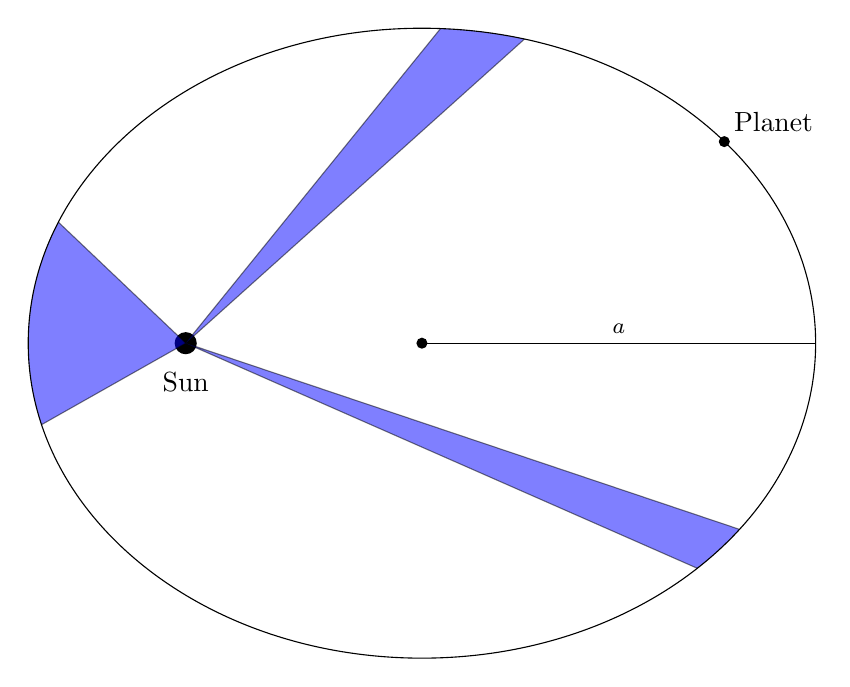
\begin{tikzpicture}[scale=2]
            \fill (0,0) coordinate (O) circle (2pt) node[below =7pt] {Sun};%
            \coordinate (A1) at (50.992527:5);
            \coordinate (A2) at (41.913511:5);
            \coordinate (B1) at (136.450216:5);
            \coordinate (B7) at (-150.524111:5);
            \coordinate (C1) at (-23.749494:5);
            \coordinate (C2) at (-18.581735:5);
            \coordinate (P) at (3.42,1.28);%%
            \fill (P) circle (1pt) node[above right] {Planet};%
            
            \begin{scope}  % The blue shaded regions
              \clip \orbit;
              \filldraw[fill=blue,opacity=0.5] (O) -- (A1) -- (A2) -- cycle;
              \filldraw[fill=blue,opacity=0.5] (O) -- (B1) -- (B7) -- cycle;%
              \filldraw[fill=blue,opacity=0.5] (O) -- (C1) -- (C2) -- cycle;%
              \end{scope}
            
              % The ellipse
            \draw \orbit;
            
            \draw (1.5,0) coordinate (M) --node[above]{\footnotesize $a$}  (4,0);
            \fill (M) circle (1pt);
        \end{tikzpicture}
        \caption{Kepler's second law}
    \end{figure}
    \FloatBarrier
    
    From figure \ref{fig:keplers-second-law}, the area of the triangle is
    \begin{equation}
        \mathop{\mathrm{d}A} = \frac{1}{2} r v_{\theta} \mathop{\mathrm{d}t}
    \end{equation}
    where $v_{\theta}$ is the transverse component of velocity in plane polar coordinates, so
    \begin{align}
        \mathop{\mathrm{d}A} &= \frac{1}{2} r^2 \dot{\theta} \mathop{\mathrm{d}t} \\
        \frac{\mathop{\mathrm{d}A}}{\mathop{\mathrm{d}t}} &= \frac{1}{2} r^2 \dot{\theta} \\
        &= \frac{1}{2} \frac{\| \vec{L} \|}{m}.
    \end{align}
    Since $\| \vec{L} \|$ is constant under any central force (such as gravitation), it implies that $\dot{A}$ is constant. Hence we have Kepler's second law.
    
    \begin{figure}[h!]
        \centering
        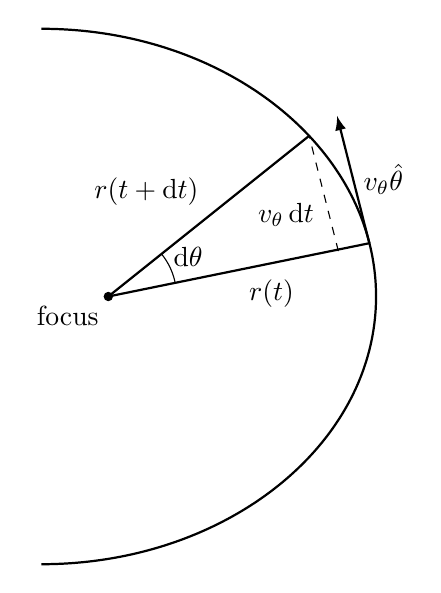
\begin{tikzpicture}[scale=0.85]
            \draw[rotate=180, thick] (0,-4) arc(270:90:5 and 4);
            \fill (1,0) circle[radius=2pt] node[below left] {focus};
            \draw[thick] (1,0) -- (4.9, 0.796) node[midway, below right] {$r(t)$};
            \draw[thick] (1,0) -- (4, 2.4) node[midway, above left] {$r(t + \mathop{\mathrm{d}t})$};
            \draw[thick, ->, arrows={-latex}] (4.9,0.796) -- (4.417,2.7) node[midway, right] {$v_{\theta} \hat{\theta}$};
            \draw[dashed] (4.437,0.678) -- (4,2.4) node[midway, below left] {$v_{\theta} \mathop{\mathrm{d}t}$};
            \draw (2,0.198) arc [start angle=11.130, end angle=38.668, radius=1] node[midway, pos=0.9, right] {$\mathop{\mathrm{d}\theta}$};
        \end{tikzpicture}
        \caption{Kepler's second law diagram}
        \label{fig:keplers-second-law}
    \end{figure}
    \FloatBarrier
    
    \item $(\text{Period of rotation})^2 \propto (\text{semi-major axis})^3$, or more commonly written as $T^2 \propto a^3$. 
    
    Let us start with Kepler's second law,
    \begin{equation}
        \frac{\mathop{\mathrm{d}A}}{\mathop{\mathrm{d}t}} = \frac{1}{2m_2} \| \vec{L} \|,
    \end{equation}
    since the right hand side is constant, the total area swept out in an orbit is
    \begin{equation}
        A = \frac{T}{2m_2} \| \vec{L} \|.
    \end{equation}
    We can use the standard expression for the total area of an ellipse, $A = \pi ab$, where $a$ and $b$ are the semi-major and semi-minor axes respectively. 
    \begin{equation}
        \label{eq:kepler-third-1}
        \frac{\pi a b }{T} = \frac{1}{2m_2} \| \vec{L} \|
    \end{equation}
    The relationship between the semi-major and minor axes is
    \begin{equation}
        \label{eq:kepler-third-2}
        b^2 = a^2 (1-e^2).
    \end{equation}
    Combining equations \ref{eq:conic}, \ref{eq:conic-h} and $k = -Gm_1m_2$ gives
    \begin{equation}
        r = \frac{\| \vec{L} \|^2}{G m_1 m_2^2 (1 + e\cos \theta)},
    \end{equation}
    which holds for every point o the ellipse. At perihelion, when $\theta = 0$, we have
    \begin{equation}
        a(1 - e) = \frac{\| \vec{L} \|^2}{G m_1 m_2^2 (1 + e)}.
    \end{equation}
    where $m_1$ is the mass of the object that exerts the gravitational force on $m_2$. Rearranging this gives
    \begin{align}
        a(1 - e)G m_1 m_2^2 (1 + e) &= \| \vec{L} \|^2, \\
        G m_1 a (1 - e^2) &= \frac{\| \vec{L} \|}{m_2^2}.
        \label{eq:kepler-third-3}
    \end{align}
    Squaring equation \ref{eq:kepler-third-1} and substituting \ref{eq:kepler-third-2} and \ref{eq:kepler-third-3} yields
    \begin{align}
        \frac{\pi^2 a^2 b^2}{T^2} &= \frac{1}{4m_2^2} \| \vec{L} \| \\
        \frac{\pi^2 a^2 a^2(1-e^2)}{T^2} &= \frac{a(1-e^2)Gm_1}{4},
    \end{align}
    hence
    \begin{equation}
        \frac{4 \pi^2}{Gm_1} a^3 = T^2,
    \end{equation}
    which is Kepler's third law.
\end{enumerate}

\section{Periodic Motion}

\subsection{Simple Harmonic Motion}

Consider a particle of mass $m$ attached to a light (massless) spring with a displacement $\vec{s}$ from the equilibrium (unstretched) position $\vec{s} = 0$ as shown in figure \ref{fig:sho}. Positive $\vec{s}$ means extension and negative $\vec{s}$ means compression of the spring. 
\begin{figure}[h!]
    \centering
    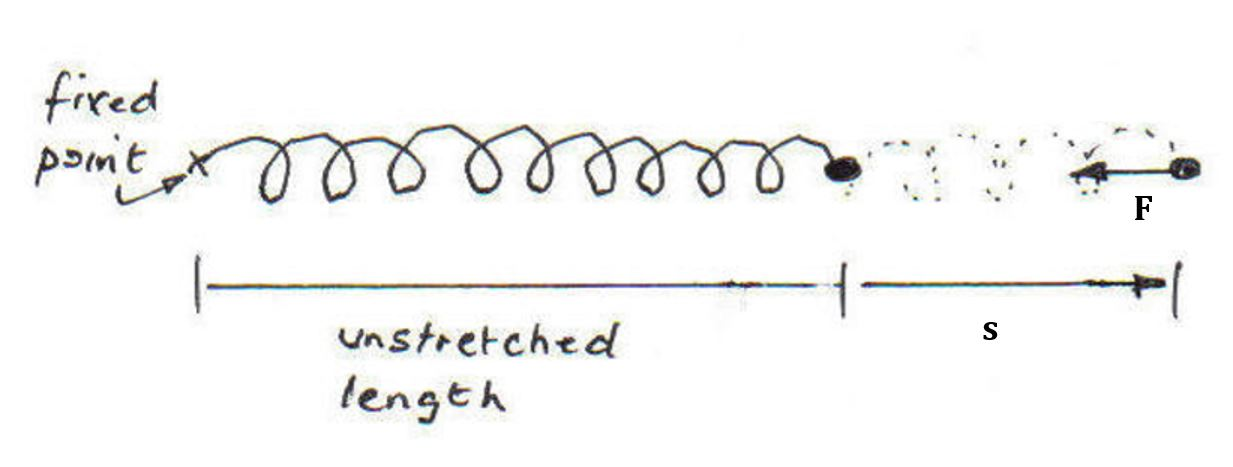
\includegraphics[scale=0.5]{notes/images/SHO.JPG}
    \caption{A simple harmonic oscillator}
    \label{fig:sho}
\end{figure}
\FloatBarrier

The so-called \textbf{restoring force}, a force that acts in the opposite direction to the displacement from the equilibrium position, is given by Hooke's Law (provided the spring obeys Hooke's law); if the Hooke's law is obeyed then the device is called a \textbf{simple harmonic oscillator} (often abbreviated to \textit{sho}) and the motion of the device is known as \textbf{simple harmonic motion} (abbreviated to \textit{shm}). Since we're only considering simple harmonic oscillators, the restoring force is $\vec{F} = -k \vec{s}$. So the equation of motion is
\begin{equation}
    \label{eq:shm-diff-eq-1}
    \vec{F} = - k \vec{s} = m \frac{\mathop{\mathrm{d}^2 \vec{s}}}{\mathop{\mathrm{d}t^2}}
\end{equation}
or, 
\begin{equation}
    \label{eq:shm-diff-eq-2}
    \frac{\mathop{\mathrm{d}^2 \vec{s}}}{\mathop{\mathrm{d}t^2}} + \frac{k}{m} \vec{s} = 0
\end{equation}
This is a second order, linear differential equation and can be solved via an auxiliary equation; Firstly, since $\vec{s}$ is in one dimension, we can assume that solutions exist of the form $\vec{s} = \eta \exp(\alpha t)$, where $\eta$ and $\alpha$ are constants.  So we have
\begin{align*}
    \frac{\mathop{\mathrm{d}^2 \vec{s}}}{\mathop{\mathrm{d}t^2}} + \frac{k}{m} \vec{s} &= \eta \alpha^2 \exp (\alpha t) + \eta \frac{k}{m} \exp(\alpha t) \\
    &= \eta \exp (\alpha t) \left(\alpha^2 + \frac{k}{m}\right) = 0
\end{align*}
So our auxiliary equation is 
\begin{equation*}
    \alpha^2 + \frac{k}{m} = 0,
\end{equation*}
giving 
\begin{equation*}
    \alpha = \pm \sqrt{\frac{k}{m}} i,
\end{equation*}
or, writing the \textbf{angular frequency} as $\omega = \sqrt{k / m}$, we have
\begin{equation*}
    \alpha = \pm \omega i
\end{equation*}
So the general solution for $\vec{s}$ is
\begin{equation}
    \vec{s} = A \cos \omega t + B \sin \omega t,
\end{equation}
where $A$ and $B$ are constants of integration of the second-order differential equation in \ref{eq:shm-diff-eq-2}. The solution can also be written in the form
\begin{equation}
    \vec{s} = C \exp \left(i \omega t \right) + D \exp \left( -i \omega t \right),
\end{equation}
where $C$ and $D$ are two arbitrary constants of integration, or as 
\begin{equation}
    \vec{s} = r \sin \left( \omega t + \phi \right).
\end{equation}
with amplitude $r$ and an arbitrary phase angle $\phi$. 

We briefly mentioned angular frequency in the equations above, however let us now formally define it. The \textbf{angular frequency} $\omega$ is defined as the range of change of the phase angle $\phi$; mathematically, we have
\begin{equation}
    \omega = \frac{\mathop{\mathrm{d}\phi}}{\mathop{\mathrm{d}t}}.
\end{equation}
But, this definition provides no physical meaning. Angular frequency (related to angular velocity) is great for systems that rotate or revolve, but our system is oscillating, so we tend to avoid this definition of $\omega$ and define it in terms of coefficients grounded in physical reality (such as frequency).  

A \textbf{periodic system} is one in which the time between repeated events is constant, The time between repeating events in a periodic system is called a \textbf{period}, denoted as $T$. Mathematically, it's the time $t$ per number of events $n$;
\begin{equation}
    T = \frac{t}{n},
\end{equation}
measured in \textbf{seconds} ($s$). \textbf{Frequency} is defined as the rate at which a periodic event occurs, denoted as $f$. Mathematically, it's the number of events $n$ per time $t$;
\begin{equation}
    f = \frac{n}{t},
\end{equation}
measured in \textbf{Hertz} ($Hz$). Note that frequency and period are reciprocals of each other, that is
\begin{equation*}
    f = \frac{1}{T} \hspace{3mm} \iff \hspace{3mm} T = \frac{1}{f}.
\end{equation*}

Angular frequency is \textit{dimensionally} defined as the number of radians per second, whereas frequency is dimensionally defined as the number of events per second, A sequence of repeated events is called a cycle. The sine function has a period of $2 \pi$ and therefore the simple harmonic oscillator repeats itself after it has moved through a single cycle of simple harmonic motion. So we have
\begin{align*}
    \omega = \frac{\phi}{t} &= \frac{2\pi \text{ radian}}{1 \text{ period}} \\
    f = \frac{n}{t} &= \frac{1 \text{ cycle}}{1 \text{ period}}
\end{align*}
Dividing one equation by the other, yields 
\begin{equation*}
    \frac{\omega}{f} = 2 \pi,
\end{equation*}
and thus
\begin{equation}
    \omega = 2\pi f = \frac{2 \pi}{T}.
\end{equation}
So the (preferred) general solution to the simple harmonic oscillator is
\begin{equation}
    \vec{s} = A \sin (2 \pi ft + \phi), 
\end{equation}
where $\vec{s}$ is displacement from the equilibrium position measured in metres, $A$ is amplitude of the simple harmonic motion measured in metres, $f$ is the frequency of the simple harmonic oscillator measured in Hertz and $\phi$ is the phase of the simple harmonic oscillator. Substituting this solution into the original differential equation \ref{eq:shm-diff-eq-1}, we find that
\begin{equation*}
    \frac{k}{m} = 4 \pi^2 f^2,
\end{equation*}
solving for frequency and time period gives
\begin{equation*}
    f = \frac{1}{2\pi} \sqrt{\frac{k}{m}} \hspace{3mm} \text{and} \hspace{3mm} T = 2 \pi \sqrt{\frac{m}{k}}.
\end{equation*}
So angular frequency can be defined in terms of the particle's mass and the spring constant
\begin{equation}
    \omega = \sqrt{\frac{k}{m}}.
\end{equation}
We should also note that the frequency and time period do not affect the amplitude, so a sho oscillating with a large amplitude will have the same frequency and period as an identical sho oscillating with a smaller amplitude.

The velocity of the particle can be found by considering the first time derivative of displacement, so we have
\begin{equation}
    \vec{v} = \frac{\mathop{\mathrm{d}\vec{s}}}{\mathop{\mathrm{d}t}} = \frac{\mathrm{d}}{\mathop{\mathrm{d}t}} (A \sin(2\pi ft + \phi)) = 2 \pi f A \cos(2\pi f t + \phi).
\end{equation}
Applying $\omega = 2\pi f$ and $\sin^2 \theta + \cos^2 \theta \equiv 1$ to the equation above yields an equation for speed $v$;
\begin{equation*}
    v = \pm \omega \sqrt{A^2 - \| \vec{s} \|^2},
\end{equation*}
For acceleration, we could take the derivative of velocity with respect to time, however, if we consider the differential equation in \ref{eq:shm-diff-eq-1}, we quickly see that
\begin{equation*}
    m \vec{a} = - k \vec{s},
\end{equation*}
so 
\begin{equation}
    \vec{a} = - \omega^2 \vec{s} = -\omega^2 A \sin(2 \pi f t + \phi).
\end{equation}

\subsection{Potential and Kinetic Energy in Simple Harmonic Motion}

We now consider the variations of the potential energy and kinetic energy of the particle as it undergoes simple harmonic motion. The force $\vec{F} = - k \vec{s}$ is a conservative force so the elastic potential energy $E_p$ is 
\begin{equation}
    E_p = \frac{1}{2} k \| \vec{s} \|^2 + E_{p, 0},
\end{equation}
where $E_{p,0}$ denotes the potential energy at the equilibrium position $\vec{s} = 0$. We can choose $E_{p, 0} = 0$ $J$ and so the potential energy is given by
\begin{equation}
    E_p = \frac{1}{2} k \| \vec{s} \|^2 = \frac{1}{2} k A^2 \sin^2 (\omega t + \phi) = \frac{1}{2} k A^2 \sin^2 (2 \pi f t + \phi)
\end{equation}
The kinetic energy $E_k$ or the particle is given by
\begin{equation}
    E_k = \frac{1}{2} m \| \vec{v} \|^2 = \frac{1}{2}m \omega^2 A^2 \cos^2(\omega t + \phi) = 2 \pi^2 m f^2 A^2 \cos^2 (2 \pi f t + \phi)
\end{equation}

\noindent The total energy of the system $E$ is $E = E_k + E_p$, so
\begin{equation}
    E = \frac{1}{2} m \omega^2 A^2 \cos^2 (\omega t + \phi) + \frac{1}{2} k A^2 \sin^2 (\omega t + \phi),
\end{equation}
but $\omega^2 = k / m$, so
\begin{align*}
    E &= \frac{1}{2} m A^2 \frac{k}{m} A^2 \cos^2 (\omega t + \phi) + \frac{1}{2} k A^2 \sin^2 (\omega t + \phi) \\
    &= \frac{1}{2} k A^2 \left[\sin^2(\omega t + \phi) + \cos^2(\omega t + \phi)\right],
\end{align*}
hence, 
\begin{equation}
    E = E_k + E_p = \frac{1}{2}kA^2. 
\end{equation}

\subsection{Damped Oscillations}

In all \textbf{real} mechanical oscillators there is some form of \textbf{damping} (or resistive force acting on the system). The damping force opposes the motion of the particle. Consider a damping force that is proportional to velocity of the particle, i.e. $\vec{F}_f = -b \vec{v}$ with a positive constant $b$. Suppose the velocity is positive (parallel to positive $\vec{s}$), then the damping force is in the opposite direction. See figure ??.

In general, a particle in simple harmonic motion has the following equation of motion
\begin{equation}
    \frac{\mathop{\mathrm{d}^2\vec{s}}}{\mathop{\mathrm{d}t^2}} = - \omega^2 \vec{s} \text{ or }
    \frac{\mathop{\mathrm{d}^2\vec{s}}}{\mathop{\mathrm{d}t^2}} + \omega^2 \vec{s} = 0.
\end{equation}
However in the case of damped harmonic motion, the equation of motion is
\begin{equation}
    \frac{\mathop{\mathrm{d}^2\vec{s}}}{\mathop{\mathrm{d}t^2}} + \frac{b}{m} \frac{\mathop{\mathrm{d}\vec{s}}}{\mathop{\mathrm{d}t} }+ \omega^2 \vec{s} = 0,
\end{equation}
or more commonly we let $\lambda = b/m$, so we have

\begin{equation}
    \frac{\mathop{\mathrm{d}^2\vec{s}}}{\mathop{\mathrm{d}t^2}} + \lambda \frac{\mathop{\mathrm{d}\vec{s}}}{\mathop{\mathrm{d}t} }+ \omega^2 \vec{s} = 0,
\end{equation}
This is a second-order, linear, homogeneous differential equation with constant coefficients $\lambda$ and $\omega^2$. So the general solution is dependent on the discriminant of the auxiliary equation
\begin{equation}
    q^2 + \lambda q + \omega^2 = 0.
\end{equation}
So we have three cases:
\begin{itemize}
    \item When $\lambda^2 - 4 \omega^2 > 0$, then the auxiliary equation has two distinct real roots and the general solution is 
    \begin{equation}
        \vec{s} = c_1 \exp(q_1 t) + c_2 \exp(q_2 t).
    \end{equation}
    This is classed as heavy damping.
    \item When $\lambda^2 - 4 \omega^2 = 0$, then the auxiliary equation has a repeated real root and the general solution is
    \begin{equation}
        \vec{s} = (c_1 t + c_2) \exp(q_1 t).
    \end{equation}
    This is classed as critical damping. 
    \item When $\lambda^2 - 4 \omega^2 < 0$, the the auxiliary equation has two distinct complex roots and the general solution is
    \begin{equation}
        \vec{s} = \exp\left(-\frac{\lambda}{2}t\right) \left[c_1 \sin \left(\frac{\alpha}{2}t\right) + c_2 \cos \left(\frac{\alpha}{2}t\right)\right]   ,
    \end{equation}
    where $\alpha^2 = 4 \omega^2 - \lambda^2$. This is classed a light damping.
\end{itemize}

\begin{figure}[h!]
    \centering
    \begin{tikzpicture}
        \draw[->] (-1,0)--(15,0) node [above left]  {$t$};
        \draw[->] (0,-4)--(0,4) node [below right]  {$\vec{s}$};
        \draw[scale=2,domain=0:7,smooth,variable=\x,blue, thick] plot ({\x}, {1.5 * exp(-1 * \x) - 0.5 * exp(-3 * \x))});
        \draw[scale=2,domain=0:7,smooth,variable=\x,red, thick] plot ({\x}, {exp(-2 * \x) * (1 + 2 * \x)});
        \draw[scale=2,domain=0:7,smooth,variable=\x,purple, thick,samples=300] plot ({\x}, {exp(-0.3 * \x) * (cos(1.5 *  deg(\x)))});
        \node[text=blue] at (13,3) {Heavy damping};
        \node[text=red] at (13.1,2.2) {Critical damping};
        \node[text=purple, ] at (12.95,1.4) {Light damping};
    \end{tikzpicture}
\end{figure}
\FloatBarrier

\subsection{Resonance}

In the absence of damping, i.e when $\lambda = 0$ or when the oscillator is said to be in \textbf{free oscillation}, the natural angular frequency of oscillation, denoted by $\omega_0$ is $\sqrt{k/m}$; similarly, the natural frequency of the oscillator denoted $f_0$ is $\omega_0/2\pi$. 

A oscillator is said to be in \textbf{forced oscillation} if there is a periodic driver force applied to the oscillator. In this case oscillator will oscillate at the frequency of the driving force, known as the \textbf{driving frequency}. 

If the driving frequency is equal to the natural frequency of the oscillator, then the oscillator will \textbf{resonate}. When the oscillator resonates, the amplitude of the oscillation increases dramatically. If the system is not damped, the amplitude will increase to the point at which the oscillator breaks / failed (i.e the glass breaks in the context of an opera singer breaking a glass with their voice). Figure \ref{fig:resonance} shows the effect of damping on forced oscillator. 

\begin{figure}[h!]
    \centering
    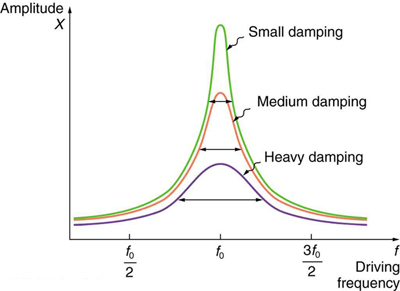
\includegraphics[scale=1.2]{notes/images/Resonance.JPG}
    \caption{Damping on a forced oscillator}
    \label{fig:resonance}
\end{figure}
\FloatBarrier


The greatest possible transfer of energy from the driver to the forced oscillator occurs at the natural frequency, hence the amplitude of the oscillator is maximum at the natural frequency. 

\subsubsection*{Examples of resonance}
\begin{itemize}
    \item \textbf{Clocks} : Clocks can keep time using the resonance of a pendulum or a quartz crystal.
    \item \textbf{Musical Instruments} : Instruments resonate to produce louder notes. 
    \item \textbf{Magnetic Resonance Imaging} : MRI uses resonance effects of hydrogen nuclei to produce diagnostic scans of the inside of our bodies. 
\end{itemize}

\section{Fluids}

\subsection{Density}

The density of a substance is it's mass per unit of volume or the ratio of mass to volume. It is a scalar quantity used to measure the substance's ``compactness''. 

\begin{definition}{(\textbf{Density})}
\textit{The density $\rho$, or the volumetric mass density, of a substance is its mass per unit of volume. Mathematically, density is defined as mass $m$ divided by volume $V$:}
\begin{equation}
    \rho = \frac{m}{V}.
\end{equation}
\textit{measured in \textbf{kilogram per cubic metres} ($kgm^{-3}$).}
\end{definition}

In A2 Physics we are required to know methods for determining density, including regular, non regular objects and fluids (specifically liquids). A regular object has faces which are standard polygons.Non regular objects are therefore those which do not have standard polygons for faces. To determine the density of an object, it's mass and volume must be recorded. The mass is normally measured with a set of digital scales or balances. We now consider the volume of regular, non regular objects and fluids;
\begin{itemize}
    \item \textbf{Fluids}: The volume of a fluid can be determined using a measuring cylinder. 
    \item \textbf{Regular objects}: The volume of a regular object can be determined using calculations based on the geometry of the object. Necessary measurements for such a calculation can be recorded using a ruler, digital calipers or micrometer. 
    \item \textbf{Non regular objects}: The volume of a non regular object can be determined using the \textit{displacement method}, which requires a measuring cylinder and a known amount of liquid (preferably water). Record the initial volume of the liquid $V_0$ in the measuring cylinder. Submerge the object in the liquid and record the new volume of the liquid $V_1$. The volume of the object $V$ can be calculated using the difference of the two recorded volumes, that is
    \begin{equation*}
        V = V_1 - V_0.
    \end{equation*}
\end{itemize} 
We can then calculate the density of the object / fluid using the equation 
\begin{equation*}
    \rho = \frac{m}{V},
\end{equation*}
where $m$ is the recorded mass and $V$ is the recorded / calculated volume. 

\subsection{Pressure}
\label{subsection:pressure}

\begin{definition}{(\textbf{Pressure})}
\textit{Pressure is the amount of force applied \textit{perpendicular} to the surface of an object per unit area over which that force is distributed (i.e. acting). Mathematically; the pressure $p$ of an object is defined as the ratio between the magnitude of the normal force $\| \vec{F}_n \|$ and the area of the surface on contact $A$, that is}
\begin{equation}
    p = \frac{\| \vec{F}_n \|}{A},
\end{equation}
\textit{measured in \textbf{pascals} (Pa).}
\end{definition}

\begin{definition}{(\textbf{Pascals})}
\textit{The SI unit for pressure, the pascal (Pa), is equal to one newton per square metre, thus}
\begin{equation*}
    [Pa] = [Nm^{-2}] = [kgm^{-1}s^{-2}].
\end{equation*}
\end{definition}

The pascal is also a unit of stress and the topics of pressure and stress are connected, however, we will discuss that in a later section. 

\subsection{Liquid Pressure}

When a person swims under the water, water pressure is felt acting on the person (specifically their eardrums). The deeper that person swims, the greater the pressure (due to the weight of the water above them). This is an example of a liquid exerting pressure on a solid.

Liquids exert pressure on solids, since the surfaces of the solids are bombarded by the liquids molecules, thus exerting a force on the surface of the solid. Liquid pressure is dependent of the depth (see introduction). In a similar fashion, it also depends on the density of the liquid. If someone was submerged in a liquid more dense than water, the pressure would be greater, thus we say that depth, density and liquid pressure are directly proportionate. 

\begin{theorem}
\textit{The pressure due to a liquid in liquid columns of constant density or at a depth within is given by the following relationship}
\begin{equation}
    p = \rho \| \vec{g} \| h,
\end{equation}
\textit{where $p$ is liquid pressure, $\| \vec{g} \|$ is the magnitude of acceleration due to gravity, $\rho$ is the density of the liquid and $h$ is the height of the liquid column or depth within a substance.}
\begin{proof}
\textit{Consider an area $A$ at the bottom of a vessel of liquid of height $h$. The weight of the column of liquid directly above this area $\vec{W}$ produces pressure. From this we have}
\begin{equation*}
    \vec{W} = m\vec{g} \textit{ and } \rho = \frac{m}{V} \textit{ and } V = Ah,
\end{equation*}
\textit{where $m$ is the mass and $V$ is the volume of the liquid in the vessel. Combining these equations gives us}
\begin{equation*}
    \vec{W} = A h \rho \vec{g}. 
\end{equation*}
\textit{The we have}
\begin{equation*}
    p = \frac{\| \vec{W} \|}{A} = \frac{Ah\rho \| \vec{g} \|}{A}.
\end{equation*}
\textit{With the area in the numerator and the area in the denominator cancelling each other out, we are left with}
\begin{equation*}
    p = \rho \| \vec{g} \| h.
\end{equation*}
\end{proof}
\end{theorem}

\subsection{Buoyancy}

Archimedes was commission by the King of Syracuse to determine if a golden crown was made for him was made of pure gold or a low grade alloy. As the story goes, Archimedes was in his bath, when he immersed himself in the water and felt a bit lighter. He realized, that this buoyant force he was experiencing could be used to determine the quality of the king's crown. 

\begin{theorem}{\textbf{(Archimedes' Principle)}}
\textit{The magnitude of the buoyant force $\vec{B}$ on an object immerse in a fluid is equal to the magnitude of weight of the fluid displaced.}
\begin{proof}
\textit{Consider an immerse prism/cylinder with a cross-sectional area $A$. The buoyant force $\vec{B}$ is the resultant force and can be explained in terms of pressure differences.}
\begin{align*}
    \| \vec{B} \| &= \| \vec{F}_{bottom} \| - \| \vec{F}_{top} \| \\
    &= (p_{bottom} - p_{top}) A \\
    &= (\rho \| \vec{g} \| h_{bottom} - \rho \| \vec{g} \| h_{top}) A \\
    &= (h_{bottom} - h_{top}) \rho \| \vec{g} \| A \\
    &= \Delta h A \rho \| \vec{g} \| \\
    &= \rho \| \vec{g} \| V \\
    &= m_{fluid} \| \vec{g} \| \\
    &= \| \vec{W}_{fluid} \|
\end{align*}
\textit{where $\rho$ is the density of the liquid, $\Delta h$ is the height difference between the bottom and top of the prism/cylinder.}
\end{proof}

An object will sink if the buoyant force is less than the weight of the object. We can determine whether an object will sink or float by considering it's apparent weight $\vec{W}'$ in a one-dimensional model. Let us first define our directions in $\mathbb{R}$. Any force acting upwards will be negative ($-$) and downwards force will be positive ($+$). So the apparent weight of an object immersed in a fluid is given by 
\begin{align*}
    \vec{W}' &= \vec{W} - \vec{B} \\
    &= m_{object} \| \vec{g} \| - m_{fluid} \| \vec{g} \| \\
    &= (\rho_{object} V - \rho_{fluid} V) \| \vec{g} \| \\
    &= (\rho_{object} - \rho_{fluid}) \| \vec{g} \| V 
\end{align*}
So when;
\begin{itemize}
    \item $\rho_{object} > \rho_{fluid}$ the apparent weight is positive and the object sinks 
    \item $\rho_{object} \leq \rho_{fluid}$ the apparent weight is less than or equal to zero and the object floats.
\end{itemize}
So icebergs float as the density of ice is less than the density of water (which is counter-intuitive if we consider the kinetic model, see section \ref{subsection:kinetic-model}). 
\end{theorem}

\subsection{Drag}
\label{subsection:drag}

The force on an object that resists its motion through a fluid is called drag or viscous friction, denoted $\vec{F}_d$. When the fluid is a gas, like air, it is called aerodynamic drag (or more commonly, air resistance). When the fluid is a liquid, like water, it is called hydrodynamic drag. The ``drag'' equation, derived from Bernoulli's equation for the pressure in a fluid, is 
\begin{equation}
    \| \vec{F}_d \| = \frac{1}{2}\rho C_d A \vec{v} \cdot \vec{v},
\end{equation}
where $C_d$ is the so-called coefficient of drag. We won't derive this equation, but let's take the equation apart to consider why these factors affect drag.
\begin{itemize}
    \item Drag increases with the \textit{density} of the fluid $\rho$. More density, means more mass, hence more momentum, which means more resistance to getting out of the way. The two quantities are directly proportional
    \begin{equation*}
        \| \vec{F}_d \| \propto \rho.
    \end{equation*}
    \item Drag increases with area $A$, what we mean by area is the cross sectional area of the object in the direction of motion. From liquid relationship, we know the force acting on an object due to pressure is proportional to the cross-sectional area. We should note that the liquid pressure relationship can be extrapolated for other fluids such as gases. So the two quantities are directly proportional
    \begin{equation*}
        \| \vec{F}_d \| \propto A.
    \end{equation*}
    \item Drag increases with speed $\| \vec{v} \|$. This should be self-evident. However as drag is a complex phenomena, there are situations where drag is proportional to some power of speed such a one, two or $n$. Most commonly we use speed squared, however in a situation described later on we will use a power of one. Recall that speed is the derivative of distance with respect to time. Solving nonlinear differential equations is extremely tedious, so we usually adopt a simpler model of drag than the ``drag equation''. 
    \begin{equation*}
        \| \vec{F}_d \| \propto \| \vec{v} \|^n
    \end{equation*}
\end{itemize}
Combining these factors will produce a similar equation to the ``drag equation''. Although this is not a proof or derivation it allows us to understand why the drag equation is an acceptable model of drag. 

\subsubsection{Terminal Velocity}

Terminal velocity is the highest velocity attainable by an object as it falls through a fluid. Mathematically, it occurs when the drag force $\vec{F}_d$ balances the downwards force of gravity, weight $\vec{W}$. 



Let us now imagine we're parachute jumper (another age old example). We jump of the drop plane and draw our free body diagram as we fall. Initially we have no velocity, there is no aerodynamic drag, we're effectively in free fall with an acceleration due to gravity of magnitude $9.8$ $ms^{-1}$ (See figure \ref{fig:terminal-velocity-1}). 

\begin{figure}[h!]
    \centering
    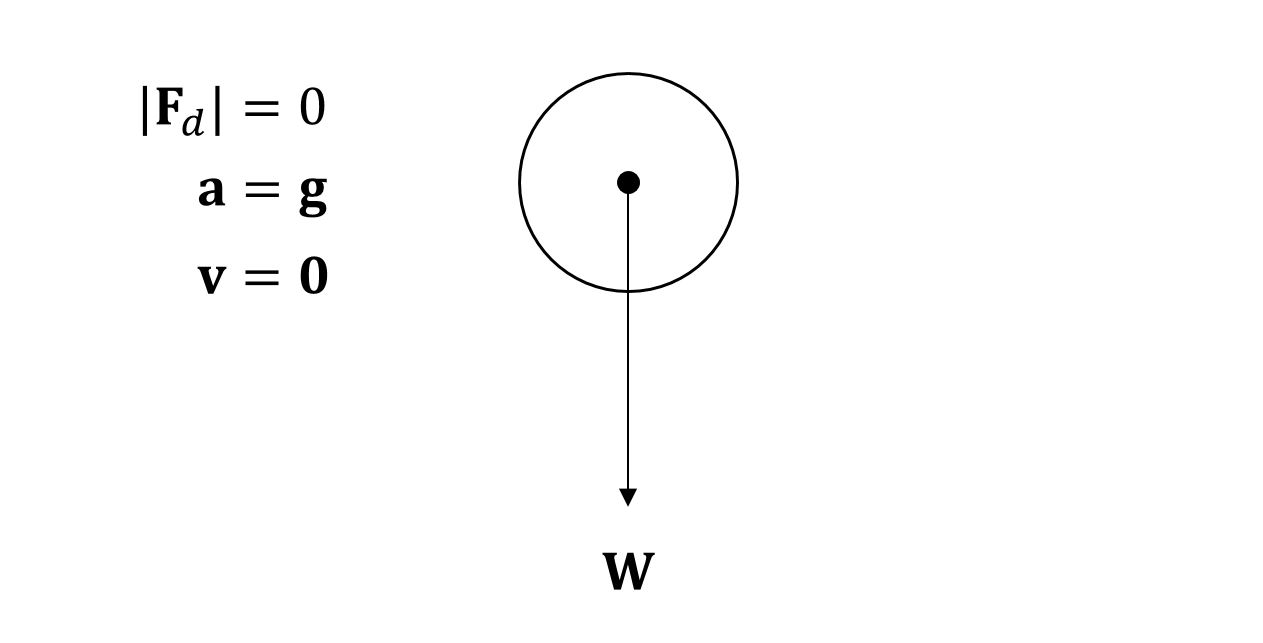
\includegraphics[scale=0.3]{notes/images/Terminal-Velocity-1.JPG}
    \caption{A free body of a sky diver: initially, pre-parachute }
    \label{fig:terminal-velocity-1}
\end{figure}
\FloatBarrier

Now it gets complicated. There is an initial acceleration, therefore an increase in velocity. With an increase in velocity comes an increase in drag and a decrease in our resultant force. This decrease in resultant force reduces acceleration (See figure \ref{fig:terminal-velocity-2}). 
\begin{figure}[h!]
    \centering
    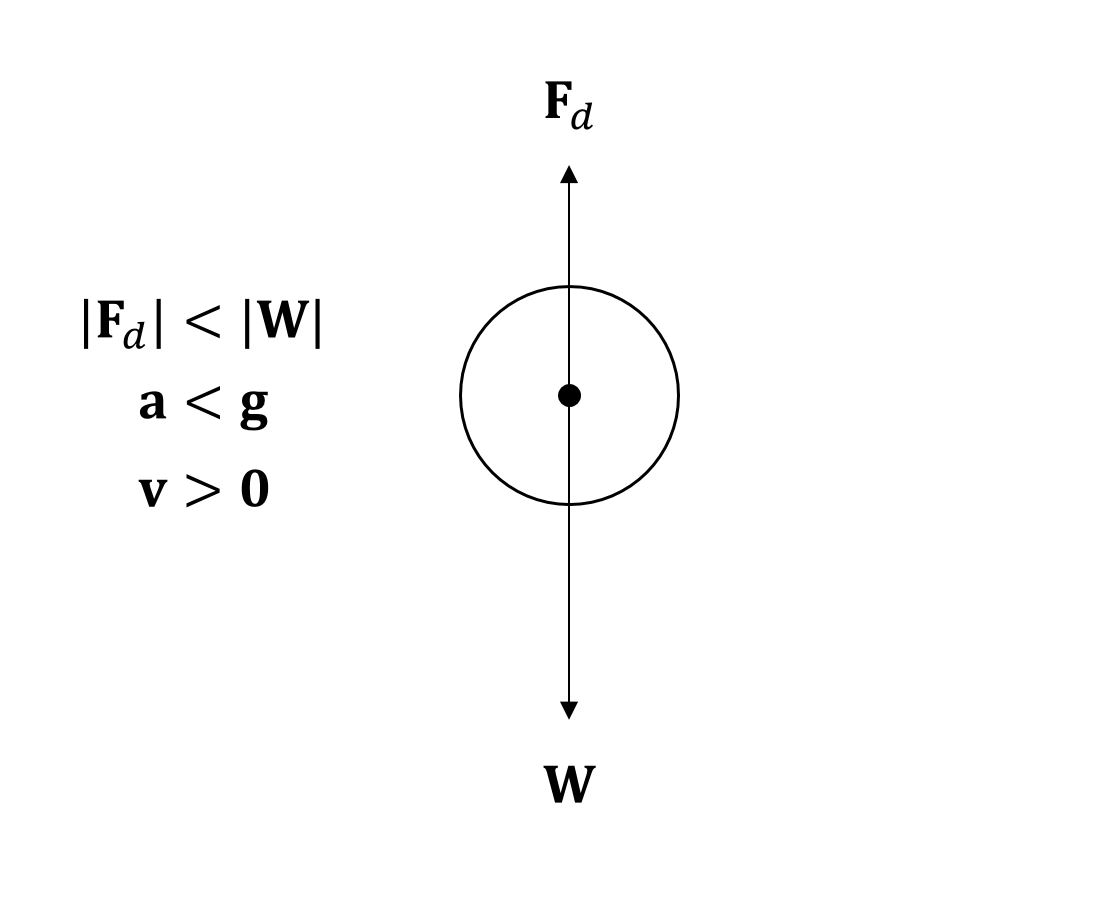
\includegraphics[scale=0.3]{notes/images/Terminal-Velocity-2.JPG}
    \caption{A free body of a sky diver: prior to terminal velocity, pre-parachute }
    \label{fig:terminal-velocity-2}
\end{figure}
\FloatBarrier
Velocity continues to increase, so does drag. As drag increases, acceleration decreases. Eventually we reach a state of equilibrium. We have reached \textit{terminal velocity}. (See figure \ref{fig:terminal-velocity-3})
\begin{figure}[h!]
    \centering
    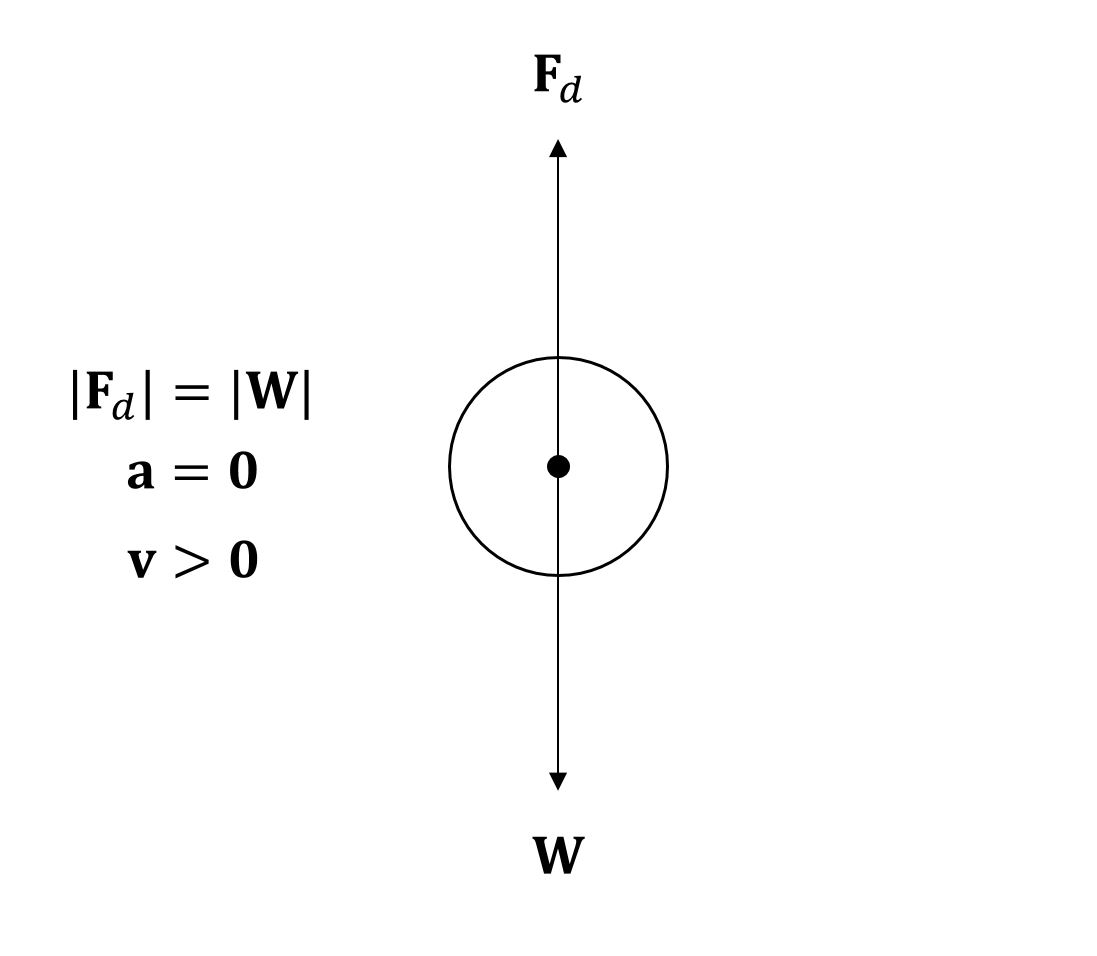
\includegraphics[scale=0.3]{notes/images/Terminal-Velocity-3.JPG}
    \caption{A free body of a sky diver: terminal velocity, pre-parachute }
    \label{fig:terminal-velocity-3}
\end{figure}
\FloatBarrier
We then open our parachute. Opening the chute significantly increases our areas, which increases drag. The upwards drag force is now greater than our weight. The resultant force and acceleration are now directed upwards (deceleration). (See figure \ref{fig:terminal-velocity-4}). 
\begin{figure}[h!]
    \centering
    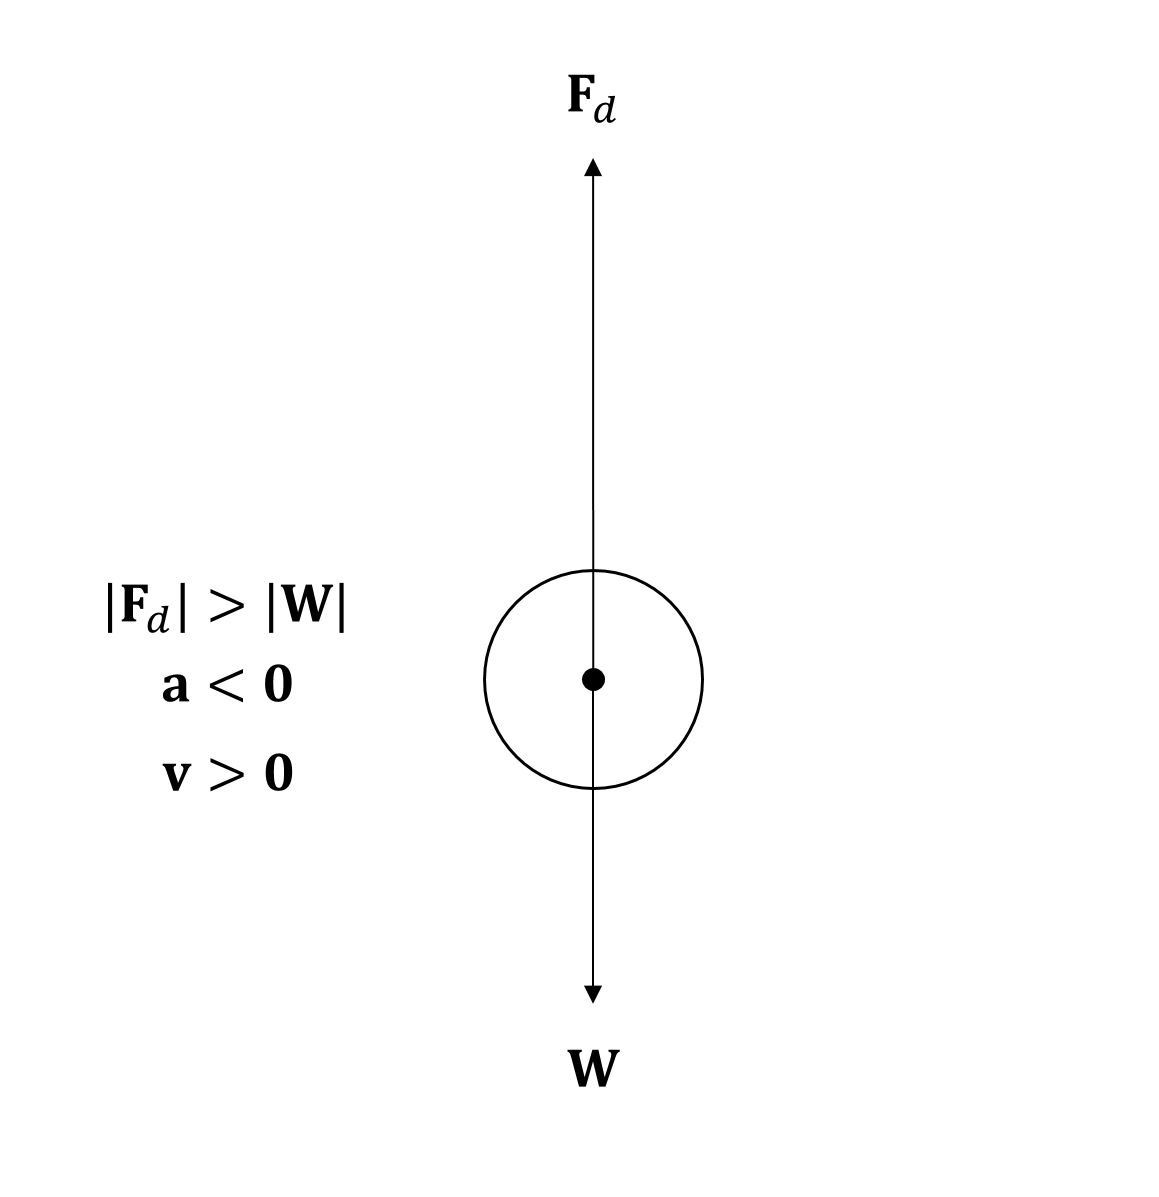
\includegraphics[scale=0.3]{notes/images/Terminal-Velocity-4.JPG}
    \caption{A free body of a sky diver: initially, post-parachute }
    \label{fig:terminal-velocity-4}
\end{figure}
\FloatBarrier
So velocity decreases, so drag decreases. Drag decreases, so the resultant force decreases. Deceleration decreases. (See figure \ref{fig:terminal-velocity-5}).
\begin{figure}[h!]
    \centering
    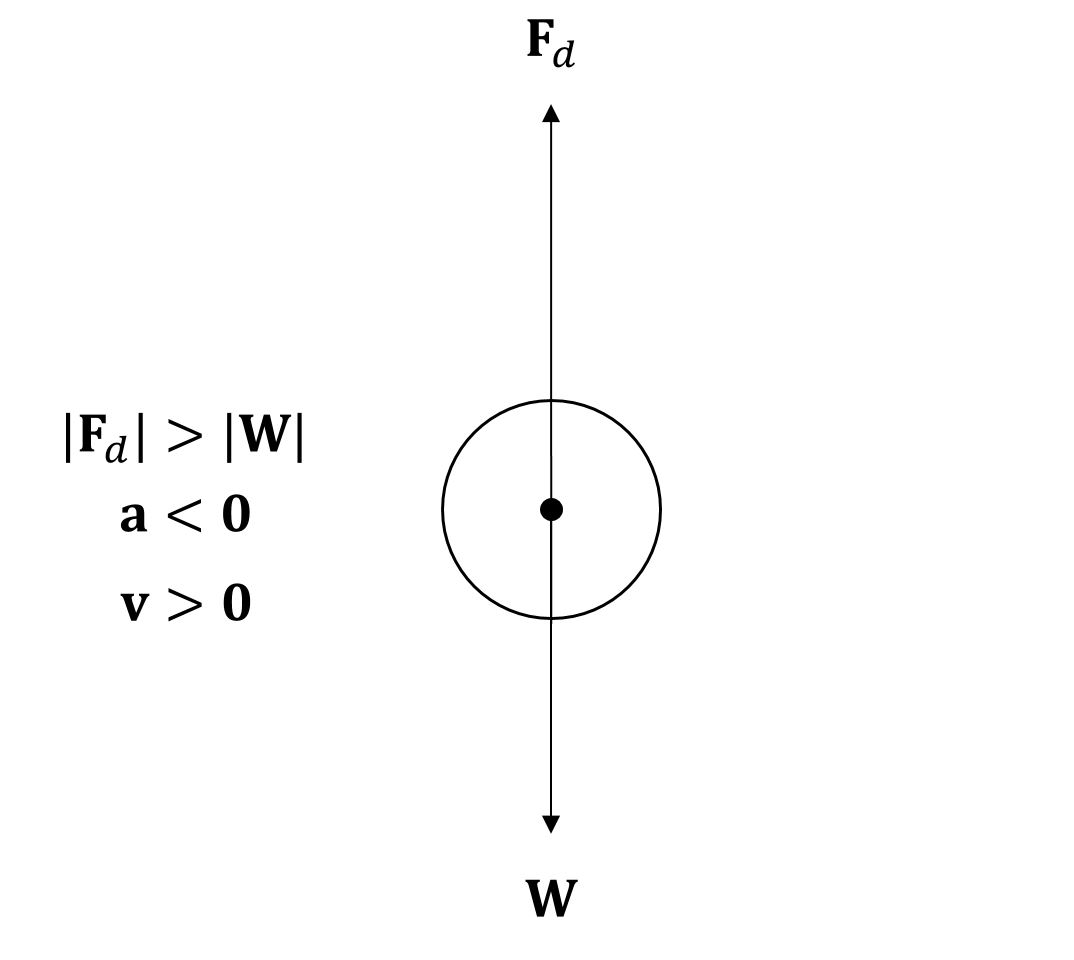
\includegraphics[scale=0.3]{notes/images/Terminal-Velocity-5.JPG}
    \caption{A free body of a sky diver: prior to terminal velocity, post-parachute }
    \label{fig:terminal-velocity-5}
\end{figure}
\FloatBarrier
Eventually we reach another state of equilibrium with a lower velocity. A different terminal velocity.
\begin{figure}[h!]
    \centering
    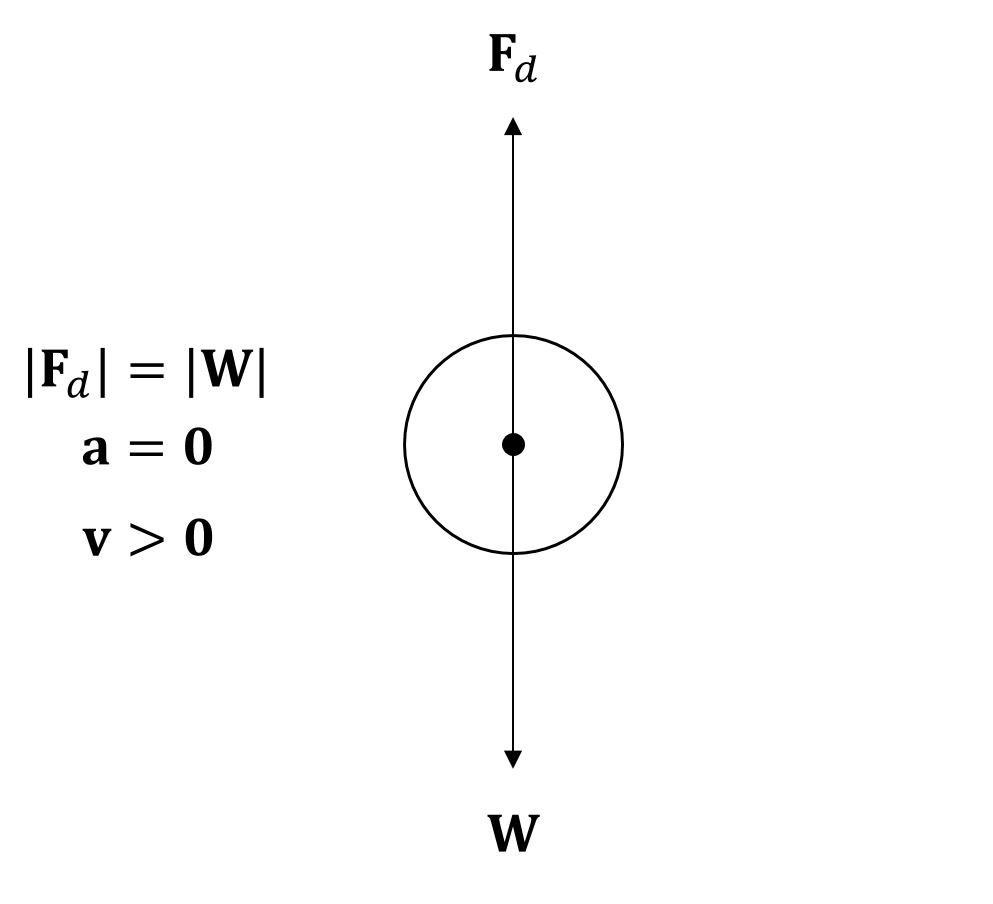
\includegraphics[scale=0.3]{notes/images/Terminal-Velocity-6.JPG}
    \caption{A free body of a sky diver: terminal velocity, post-parachute }
    \label{fig:terminal-velocity-6}
\end{figure}
\FloatBarrier

Having modelled this scenario using dynamics, lets consider an equation of motion for this scenario. As we mentioned earlier, solving non-linear differential equations is tedious, so we will use a simple model for drag.
\begin{equation*}
    \vec{F}_d = -b\vec{v}.
\end{equation*}
This allows us to quickly form an equation of motion,
\begin{equation*}
    m \frac{\mathop{\mathrm{d}\vec{v}}}{\mathop{\mathrm{d}t}} = m \vec{g} - b \vec{v}
\end{equation*}
We can solve this by introducing the integrating factor $e^{bt / m}$ to write the equation as
\begin{equation*}
    \frac{\mathrm{d}}{\mathop{\mathrm{d}t}} (e^{bt/m} \vec{v}) = e^{bt/m} \vec{g}
\end{equation*}
We now integrate, but introduce a vector integration constant $\vec{c}$. We have
\begin{equation*}
    \vec{v} = \frac{m}{t}\vec{g} + \vec{c} e^{-bt/m}
\end{equation*}
We know at time $t = 0$, the velocity is $\vec{v} = \vec{u} = \vec{0}$, so we can use this information to determine the integration constant $\vec{c}$. We get
\begin{equation*}
    \vec{v} = \frac{m}{t}\vec{g}(1 - e^{-bt/m})
\end{equation*}
Now we integrate $\vec{v}$ to determine the displacement as a function of time.  We get another integration constant, $\vec{k}$,
\begin{equation*}
    \vec{s} = \frac{m}{b}\vec{g} \left(t + \frac{m}{b} e^{-bt/m}\right) + \vec{k} 
\end{equation*}
We know, by definition, that at time $t = 0$, we have $\vec{s} = \vec{0}$. Then we have
\begin{equation*}
    \vec{s} = \frac{m}{b}\vec{g} \left(t + \frac{m}{b} e^{-bt/m} - \frac{m}{b}\right) 
\end{equation*}

\section{Examples}

\subsection{Car Stopping Distances}

This section will discuss the factors of car stopping distances, analyzing thinking distance and braking distance separately. This is a specific example of an application of physics to a scenario. Firstly, we shall define stopping distance in terms of thinking and braking distances and then consider the factors that affects them. 

\begin{definition}{(\textbf{Stopping Distance})}
\textit{The stopping distance of a car is defined as the sum of the thinking distance and the braking distance, that is}
\begin{equation*}
    \text{Stopping Distance} = \text{Thinking Distance} + \text{Braking Distance}.
\end{equation*}
\end{definition}

\begin{definition}{(\textbf{Thinking Distance})}
\textit{The thinking distance of a car is the distance travelled by the car during the driver's reaction time (time taken to engage the brakes after seeing the hazard).}
\begin{equation*}
    \text{Thinking Distance} = \| \vec{v} \|t,
\end{equation*}
\textit{where $t$ is the driver's reaction time and $\vec{v}$ is the velocity during that time period.}
\end{definition}
\begin{definition}{(\textbf{Braking Distance})}
\textit{The braking distance of a car is defined as the distance the car travels after the brakes are applied until the car is stationary. Computationally, the braking distance of a car with deceleration $\vec{a}$ and initial velocity of $\vec{u}$ $ms^{-1}$ is}
\begin{equation*}
    \text{Braking Distance} = \frac{\| \vec{u} \|^2}{2\|\vec{a}\|}.
\end{equation*}
\end{definition}

Having formally defined thinking and braking distance, we are now able to consider some of the factors that affects them. We will first consider thinking distance, then braking distance. We notice that thinking distance is dependent on two variables: velocity and reaction time. Which implies to affect thinking distance, we must consider a factor that affects one of these variables. 
\begin{itemize}
    \item The consumption of drugs and/or alcohol will increase the reaction time of the driver $t$, giving rise to an increase in thinking distance; since $t \propto \text{Thinking Distance}$. 
    \item Driver fatigue / tiredness will increase the reaction time of the driver $t$, thus increasing the thinking distance (see relationship above). 
    \item An increase in the velocity of the car during the reaction time period will increase the thinking distance, since $\| \vec{v} \| \propto \text{Thinking Distance}$.
\end{itemize}

Naturally, we can apply the same approach we did to thinking distance to discover the factors that affect braking distance, however, there are some more hidden factors. So lets start by considering the variables, as we did with thinking distance.
\begin{itemize}
    \item An increase in the initial velocity of the car $\| \vec{u} \|$ will the braking distance, since $\| \vec{u} \|^2 \propto \text{Braking Distance}$. 
    \item A decrease in the deceleration of the car $\| \vec{a} \|$ will increase the braking distance, since \\$\text{Braking Distance} \propto \frac{1}{\| \vec{a} \|}$.
\end{itemize}
We now must use concepts such as kinetic energy, work done and friction to explain the two remaining factors that affect braking distance. Firstly we shall consider whether the mass of the car $m$ affects the braking distance. By definition, the kinetic energy of the car, $E_k$, with a mass of $m$ kg and an initial velocity of $\vec{v}$ $ms^{-1}$ is 
\begin{equation*}
    E_k = \frac{1}{2} m \| \vec{v} \|^2.
\end{equation*}
To stop the car, we kinetic energy of the car must be entirely transferred to work done by friction (i.e. friction of the car and friction between of the brakes). So by the work-energy theorem, we can equate these two forms of energies
\begin{align*}
    \frac{1}{2} m \| \vec{v} \|^2 &= \vec{F} \cdot \vec{s} \\
    m &\propto \vec{s}.
\end{align*}

So the braking distance of the car is directly proportional to the mass of the car. Another consideration, is the friction between the car and the road. If the car's tires / brakes are worn or the road is wet/icy it follows that the coefficient of friction $\mu$ will decrease. Given the magnitude frictional force $\vec{F}_f$ is less than or equal to the product of the coefficient of friction and the magnitude normal reaction force $\vec{R}$, that is $\| \vec{F}_f \| \leq \mu \| \vec{R} \|$. So the frictional stopping force between the car and the road is directly proportional to the coefficient of friction. Using a similar application of the work-energy theorem, we have
\begin{equation*}
    \mu \propto \| \vec{F}_f \| \text{ and }  \vec{F}_f  \propto \frac{1}{\vec{s}}.
\end{equation*}
Note that we are working in with a one-dimensional model, so the frictional force is proportional to the magnitude of the friction force. So we conclude that $\mu \propto \frac{1}{\vec{s}}$. Hence the coefficient of friction is inversely proportional to the braking distance. 